\documentclass{article}
\usepackage{icml2017}

\usepackage{graphicx}

\usepackage{amsmath}
\usepackage{amsthm}
\usepackage{amssymb,latexsym,color}
\usepackage{mdwlist}
%\usepackage{fullpage}
%\usepackage{charter}

\usepackage{url}

%\usepackage{algorithm}
%\usepackage[noend]{algpseudocode}

%\usepackage{fullpage}
\usepackage{marvosym}
%\usepackage[techreport]{systems-cover}

\usepackage{graphicx}
\graphicspath{ {Figures/} }
\usepackage{subcaption}
%\captionsetup[subfigure]{justification=justified,singlelinecheck=false}

\newcommand{\R}{\mathsf{R}}
\newcommand{\sgn}[1]{\mbox{sgn}(#1)}
\renewcommand{\vec}[1]{\mathbf{#1}}

\def\a{{\bf a}}
\def\g{{\bf g}}
\def\x{{\bf x}}
\def\y{{\bf y}}
\def\w{{\bf w}}
\def\E{\mathbb{E}}
\def\rrow{r_\mathrm{row}}

\DeclareMathOperator*{\argmin}{argmin}

\newtheorem{lemma}{Lemma}
\newtheorem{theorem}{Theorem}
\newtheorem{claim}{Claim}
\newtheorem{corollary}{Corollary}
\newtheorem{prop}{Proposition}
\newtheorem{definition}{Definition}

\newcommand{\todo}[1]{\noindent \textbf{[TODO:] #1 } }
\usepackage{mathtools}
\DeclarePairedDelimiter\floor{\lfloor}{\rfloor}
\DeclarePairedDelimiter\ceil{\lceil}{\rceil}

\date{}

\title{Training Generalized Linear Models with End-to-end Low Precision:\\
The Cans, the Cants, plus a Little Bit Deep Learning
}

\begin{document}
\maketitle

\begin{abstract}
Allured by the recent success of training
deep learning models with end-to-end low
precision computation and data movement, 
we focus on simpler generalized linear models. 

Our positive results hold for linear
models. Although simply doing stochastic
quantization introduces innegligible bias, we are able
to develop a simple, but novel, fix 
to get an unbiased estimator of the gradient. We further 
developed an optimal quantization strategy
that minimizes the variance introduced 
by stochastic quantization. These techniques 
have been applied to a range of applications and
enabled an FPGA prototype that is up to
10$\times$ faster than using 32bit full precision.

Our negative results appear when we try
to extend our technique to non-linear models
such as SVM. We present
two different strategies with rigorous 
theoretical bounds and are able to lower the
precision by $4\times$ while still getting the same
solution. However, both fail to 
outperform a strawman quantization approach
and we analyze our observations.

Last, we also apply the optimal quantization 
strategy we developed for linear models to 
training deep neural networks with 
quantized model and achieves up to 3 points
higher accuracy than state-of-the-art BNNs
on CIFAR-10 with a standard network.
\end{abstract}

\begin{figure}[t]
\centering
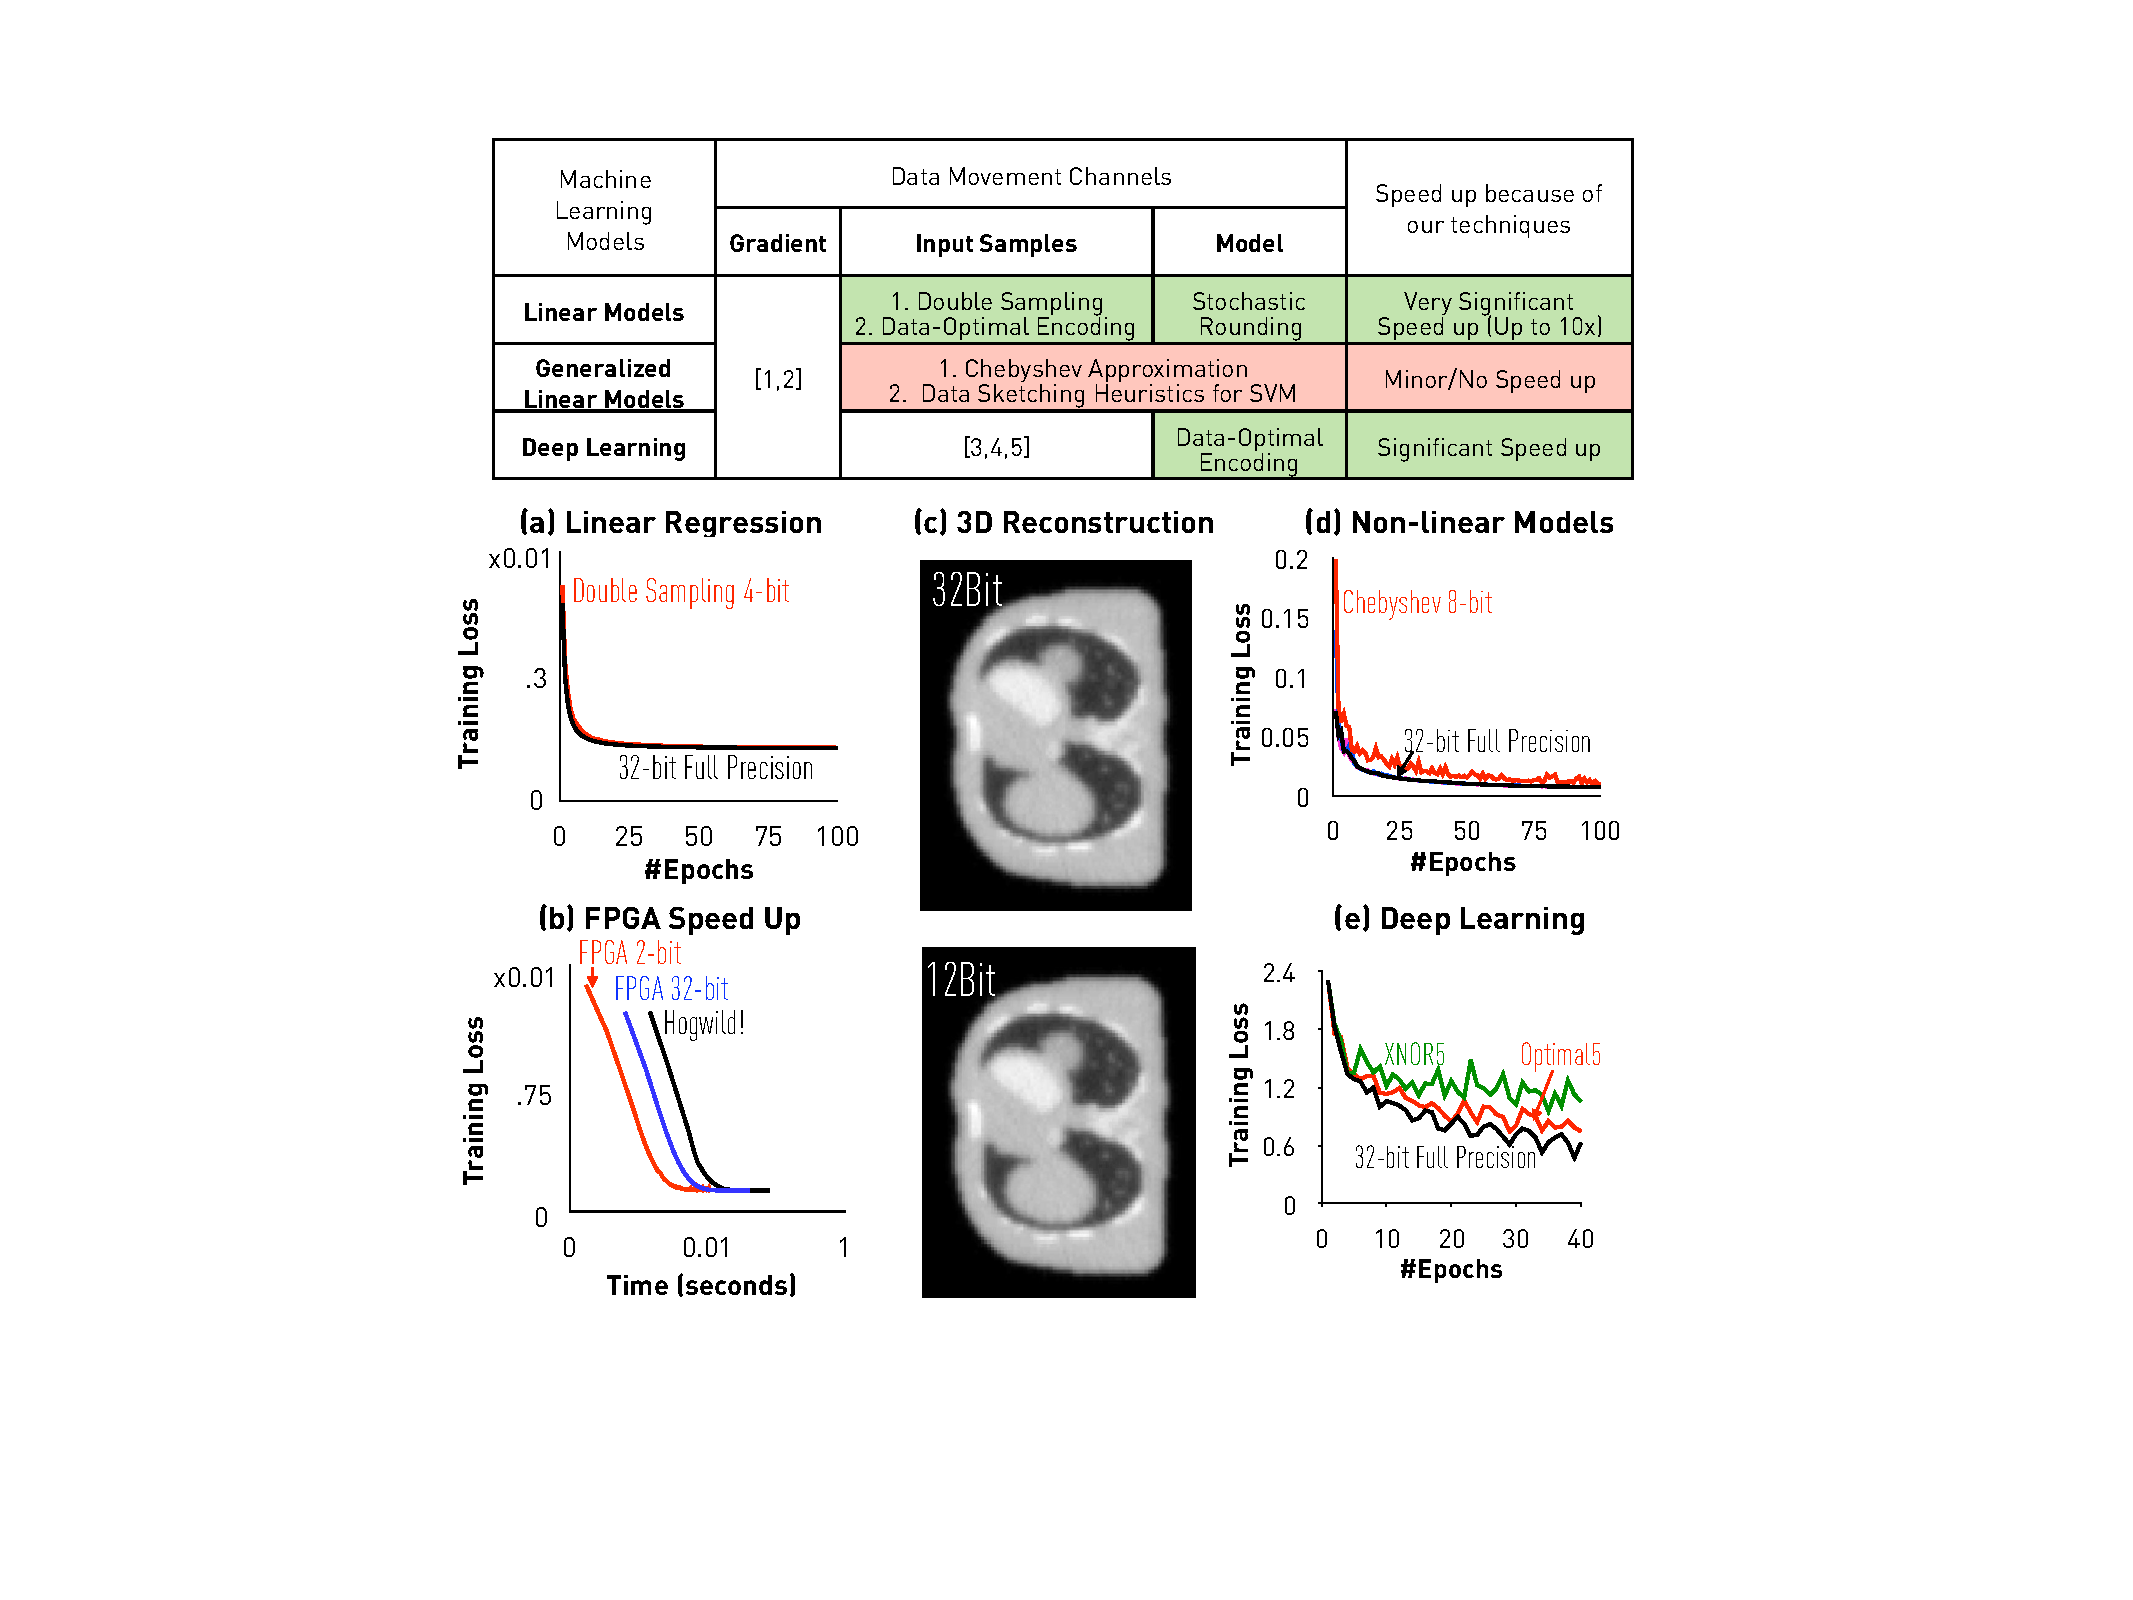
\includegraphics[width=0.5\textwidth]{Figures/RSHighlight}    
\vspace{-2em}
\caption{Overview of theoretical results and
highlights of empirical results. See
Introduction for details.}
\label{fig:highlight}
\end{figure}

%\vspace{-2em}
\section{Introduction}

For nany machine learning applications,
the total operating cost or 
power consumption are often dominated by 
the amount of data movement involved
in sending input samples and models:

\noindent
{\bf Use Case 1 (Industrial IoT).} Two
of our industry partners want to learn
linear models with data collected by sensors,
which are sent via 4G or 2G signals. To
lower the cost and power consumption 
on sensors, they want to minimize
the amount of data sent from sensors while
maintaining the training quality.

\noindent
{\bf Use Case 2. (Tomographic Reconstruction)}
One of our industry partner wants to do 
high-resolution tomographic 3D reconstruction,
in which the trained model is larger than 240GB in
32-bit precision. To scale up the system, 
they want to minimize the 
amount of data sent from the parameter server
to the worker.



All these use cases hinge on one question: {\em
When training generalized linear models,
can we lower the precision of data representation
for communicating input samples and models?}
In this paper, we develop a framework for this 
question --- In many cases, we can lower the
precision of data communication to as low as 
1 bit while getting the same training
result, both empirically and theoretically. 

\noindent
\paragraph*{Related Work on Low-precision ML.} 
Lower the precision of data representation
in machine learning systems has received
tremendous interests recently. Most of
these work try to lower the precision of
{\em gradient} in training deep learning
models~\cite{XXX,XXX,XXX,XXX,XXX,XXX,XXX,XXX,XXX}.
There are also theoretical guarantees 
that SGD will converges to the same solution~\cite{XXX,XXX,XXX}
if proper rounding strategies are applied to gradients.
For input samples and models, there have been
empirical results related to deep learning~\cite{XXX,XXX,XXX,XXX}.
For generalized linear models or tomographic reconstruction
there have been empirical studies that lower
the precision of all data representation~\cite{XXX,XXX,XXX,XXX}.
All these results, however, only hold empirically
and there are no theoretical guarantee on
the result trained with low precision
input samples and model. On the other hand,
our framework, despite its simplicity, provides
theoretical guarantees on the result.




\subsection*{Summary of Technical Contributions}

We consider the following problem in training generialized linear models: 
\begin{align}
\min_{\x}:\quad {1\over 2K}\sum_{k=1}^K l(\a_k^\top \x, b_k)^2 + R(\x)
\label{eqn:leastsquares}
\end{align}
where $l(-,-)$ is a loss function, and $R$ is a regularization term. 



The proximal stochastic gradient procedure consists in the following iterative process:
\[
\x \leftarrow \text{Prox}_{\gamma R}(\x - \gamma \g_k) := \argmin_\y {1\over 2} \|\y-(\x - \gamma \g_k)\|^2 + \gamma R(\y)
\]
where $k$ is a randomly selected sample index. The gradient at the sample $(\a_k, b_k)$ is: 
\[
\g_k := \a_k \a_k^\top \x + \a_k b_k.
\]
In the following, we denote the problem dimension by $n$. 

\vspace{-2em}
\paragraph{Related Work.} 
Thanks to its simplicity, the Stochastic Gradient Descent algorithm (SGD)~\cite{RM}, is now a standard tool in machine learning, with applications from SVM, to neural network back-propagation and recommender systems. Given its practical appeal, there has been a tremendous amount of effort invested in developing computationally efficient variants of this algorithm. 
This research field is extremely vast, see e.g.~\cite{Bottou, SVRG, Hogwild, PSGD} for examples, and a complete survey is beyond the scope of this paper. 

Here, we focus on the relatively recent efforts to understand the convergence properties of SGD in the context of low-precision data representation, such as the ones caused by fixed-point arithmetic or lossy compression. 
In particular, De Sa, Zhang, Olukotun, and Re~\cite{BUCKWILD}  proposed and analyzed BuckWild!, a variant of SGD which only employs low-precision representations. They showed that SGD can be provably robust to the rounding errors engendered by fixed-point arithmetic; in practice, BuckWild! can tolerate 8-bit integer precision, although it is observed to diverge for lower precision. 
In the same vein, recent work by Alistarh, Li, Tomioka, and Vojnovic~\cite{QSGD} proposed a family of lossy compression schemes 
allowing the optimal compression of gradient updates, while preserving the convergence properties of SGD. 
Their work was inspired by OneBit SGD, a gradient compression heuristic developed in the context of deep neural networks for speech recognition~\cite{OneBit}. 

While the above research suggests that SGD can tolerate low precision for some of its components, such as the gradient updates or the model, it leaves open the question of whether it is possible to perform end-to-end training of linear models with low-precision representations. 
In this paper, we answer this question in the affirmative, for the special case of linear regression and least squares SVM. 


\subsection{Our Results}

\paragraph{Regression.} For linear regression, we develop an algorithmic framework which allows stochastic 
quantization of data, model, \emph{and} gradient.
Empirically, as shown in Figure~\ref{fig:highlight}(a),
on datasets such as 
\texttt{cadata} dataset,\footnote{\url{https://www.csie.ntu.edu.tw/~cjlin/libsvmtools/datasets/regression.html#cadata}}
quantizing all data, model, and gradients
with 2-bit is enough to ensure convergence
to the same solution (within 0.9\%) as a standard, full-precision framework.
If the original data are stored as
32-bit floats, like in most existing
systems, our quantization decreases
the amount of data movement by up to $16\times$.
Moreover, as shown in Figure~\ref{fig:highlight}(a),
the quantized training procedure has comparable
empirical convergence rate---it requires 
almost the same number of iterations to
converge to the same loss.

\paragraph{Classification.} For classification
tasks, we studied both standard support vector
machines (SVM) and least-squares support vector
machines (LS-SVM). Our analytical results apply to both these tasks.  
As shown
in Figure~\ref{fig:highlight}(b),
on datasets such as \texttt{cod-rna},\footnote{ \url{https://www.csie.ntu.edu.tw/~cjlin/libsvmtools/datasets/binary.html#cod-rna}} quantizing all data, model, and gradients
using 2 bits per component is enough to ensure convergence
to the same solution (within 3.8\%).
When using 3-bit, we observe comparable
empirical convergence rate as
using 32-bit floating point representations.

We also investigated convergence for standard SVM (hinge loss). 
In this case, the interplay between the loss function and quantization renders convergence analysis more difficult. 
Yet, as we show in Section~\ref{sec:exp},
it is possible to develop a theoretically-sound
quantization strategy with which an end-to-end 8-bit quantization is
always sufficient to ensure robust convergence with comparable empirical
convergence rates.


\begin{figure*}[t]
\centering
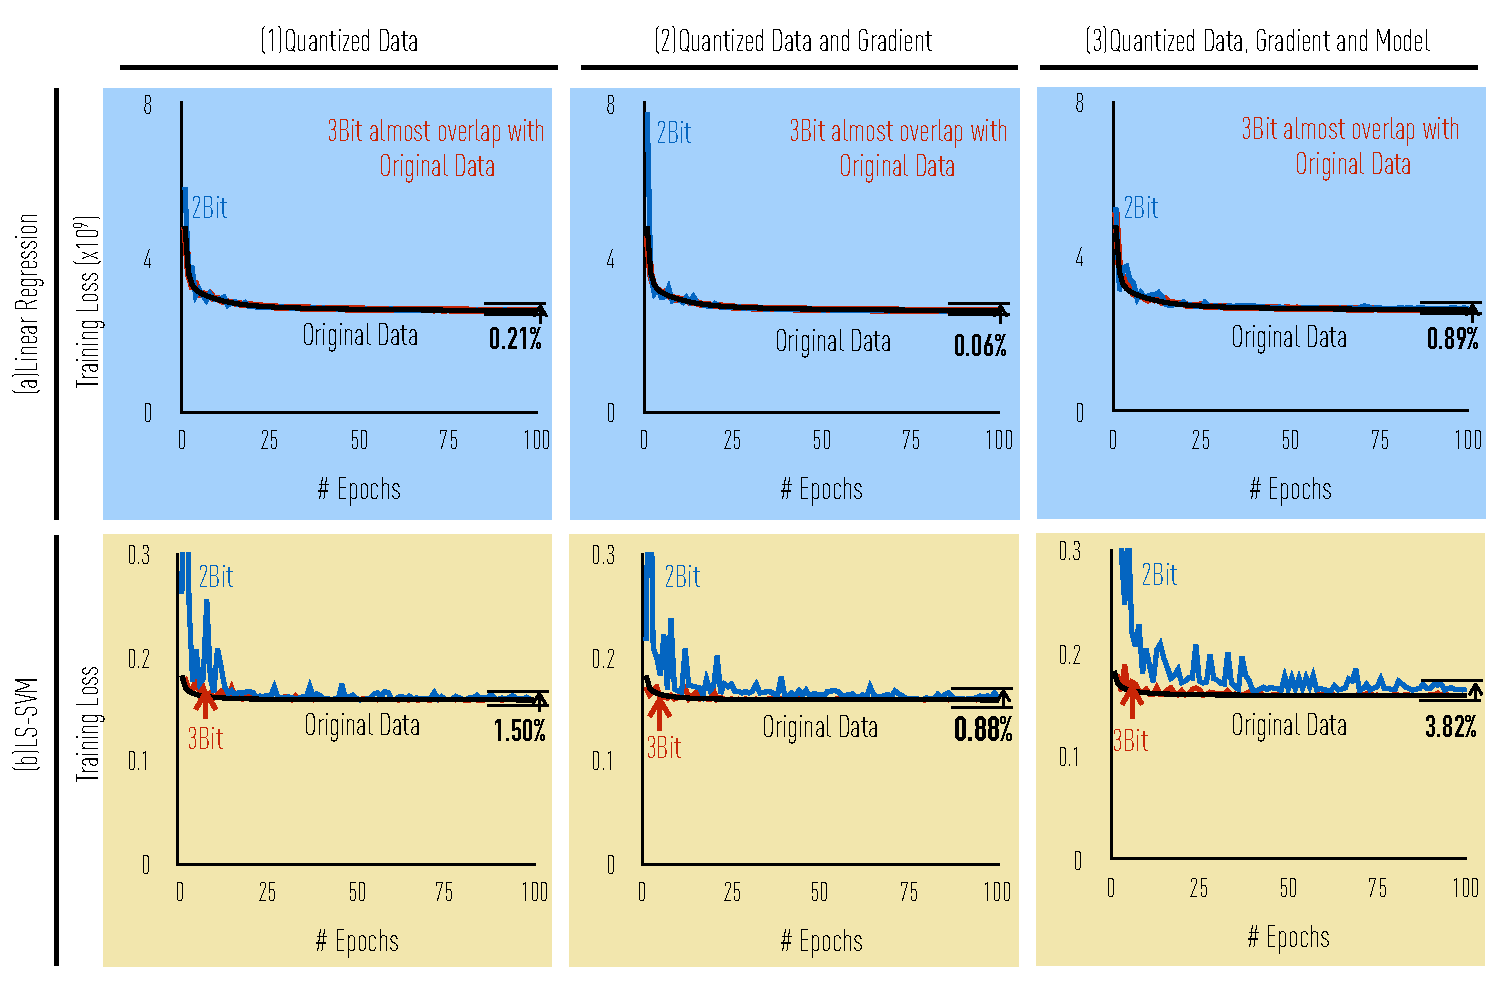
\includegraphics[width=0.85\columnwidth]{highlight-pdfcrop}    
\caption{ZipML on Linear Regression (\texttt{cadata} dataset) and LS-SVM (\texttt{cod-rna} dataset)}
\label{fig:highlight}
\end{figure*}

\section{Preliminaries}

\subsection{Computational Model}

We consider a computational model illustrated in
Figure~\ref{fig:model}.  
In this context, SGD is often bounded by the bandwidth
of data movements cross these components. 
In particular, we consider the convergence properties of the algorithm when a lossy compression scheme is applied to the data (samples), 
gradient, and model, for the purpose of reducing the communication cost of the algorithm. 
It is interesting to consider how lossy compression impacts the update step in SGD. Let $Q( \vec{v} )$ denote the compression scheme applied to a vector $\vec{v}$. 

\begin{itemize}
    \item \textbf{Original iteration}: $$\x_{t + 1} \leftarrow \x_t - \gamma \g_k (\x_t, \vec{a}_t).$$
    \item \textbf{Compressed gradient}: $$\x_{t + 1} \leftarrow \x_t - \gamma Q( \g_k (\x_t, \vec{a}_t) ).$$
    \item \textbf{Compressed model}: $$\x_{t + 1} \leftarrow \x_t - \gamma \g_k (Q(\x_t), \vec{a}_t).$$
    \item \textbf{Compressed sample}: $$\x_{t + 1} \leftarrow \x_t - \gamma \g_k (\x_t, Q(\vec{a}_t)).$$
    \item \textbf{End-to-end compression}: $$\x_{t + 1} \leftarrow \x_t - \gamma Q(\g_k (Q(\x_t), Q(\vec{a}_t))).$$
\end{itemize}










\begin{figure*}[t]
\centering   
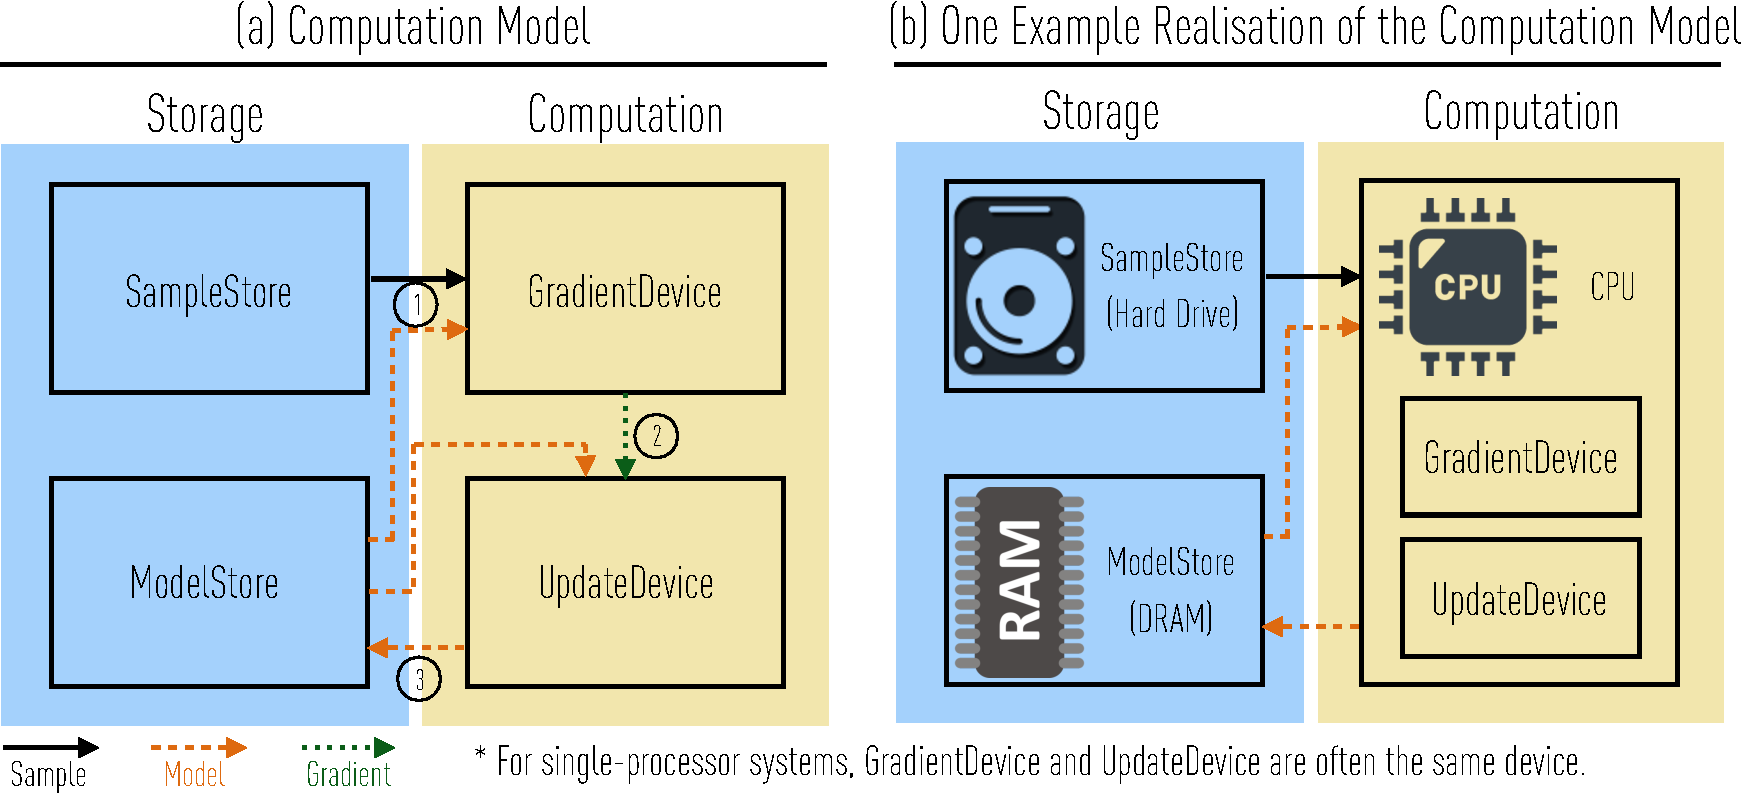
\includegraphics[scale=0.4]{compmodel-pdfcrop}
\caption{(a) A Schematic Representation of the Computation Model and (b) An Example Realisation
of the Computation Model. Three types of
data, namely (1) sample, (2) model, and (3)
gradient, moves in the system in three
steps as illustrated in (a). Given
different parameters of the computation model,
such as computational power and memory bandwidth, the system bottleneck may
vary. For example, in 
realisation (b) having a hard drive, DRAM, and a
modern CPU, it is likely that the  bottleneck when training 
a dense generalized linear model is the
memory bandwidth between SampleStore
and GradientDevice.}
\label{fig:model}
\end{figure*}






%\begin{figure}[h]
%\centering
%   
%    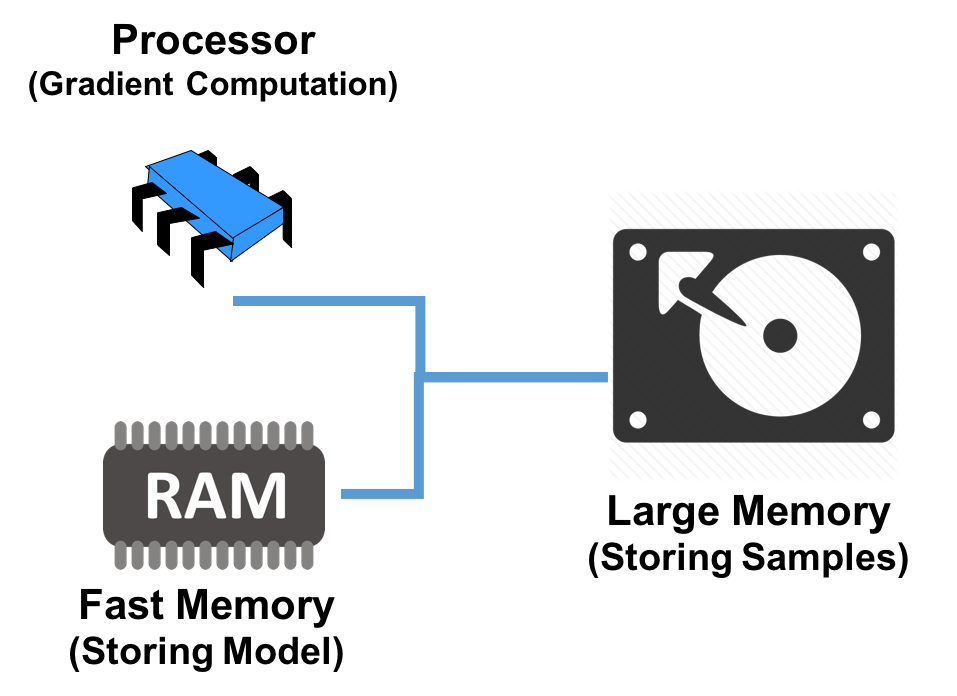
\includegraphics[scale=0.4]{schematic}
%    
%\caption{Simple Schematic of the %Computational Model}
%\label{fig:model}
%\end{figure}

\subsection{Guarantees for SGD}
In this paper we consider SGD, a general family of stochastic first order methods for finding the minima of convex (and non-convex) functions.
Due to its generality and usefulness, there is a vast literature on SGD in a variety of settings, with different guarantees in all of these settings.
Our techniques apply fairly generally in a black box fashion to many of these settings, and so for simplicity we will restrict our attention to a fairly basic setting.
For a more comprehensive treatment, see \cite{Bubeck15}.

Throughout the paper, we will assume the following setting in our theoretical analysis.
Let $\mathcal{X} \subseteq \R^n$ be a known convex set, and let $f: \mathcal{X} \to \R$ be differentiable, convex, and unknown.
We will assume the following, standard smoothness condition on $f$:
\begin{definition}[Smoothness]
Let $f: \R^n \to \R$ be differentiable and convex.
We say that it is $L$-smooth if for all $\x, \y \in \R^n$, we have
\[0 \leq f(\x) - f(\y) - \nabla f(\y)^T (\x - \y) \leq \frac{L}{2} \| \x - \y \|_2^2 \; .\]
\end{definition}

We assume repeated access to stochastic gradients, which on (possibly random) input $\vec{x}$, outputs a direction which is in expectation the correct direction to move in.
Formally:
\begin{definition}
Fix $f: \mathcal{X} \to \R$.
A \emph{stochastic gradient} for $f$ is a random function $g (\x)$ so that $\E [g (\x) ] = \nabla f( \x)$.
%A \emph{stochastic oracle} for $f$ is an oracle which on (possibly random) input $\vec{x}$, outputs a stochastic gradient for $f$ at $\vec{x}$.
We say the stochastic gradient has second moment at most $B$ if $\E [\| g \|_2^2] \leq B$ for all $\x \in \mathcal{X}$.
We say it has variance at most $\sigma^2$ if $\E [\| g (\x) - \nabla f(\x) \|_2^2] \leq \sigma^2$ for all $\x \in \mathcal{X}$. 
\end{definition}

Under these conditions, the following convergence rate for SGD is well-known:

\begin{theorem}[e.g. \cite{Bubeck15}, Theorem 6.3]
Let $\mathcal{X} \subseteq \R^n$ be convex, and let $f: \mathcal{X} \to \R$ be an unknown, convex, and $L$-smooth.
Let $\x_0 \in \mathcal{X}$ be given, and let $R^2 = \sup_{\x \in \mathcal{X}} \| \x - \x_0 \|^2$.
Suppose we run projected SGD on $f$ with access to independent stochastic gradients with variance bound $\sigma^2$ for $T$ steps, with step size $\eta_t = 1 / ( L + \gamma^{-1})$, where $\gamma = \frac{R}{\sigma} \sqrt{\frac{2}{T}}$, and
\begin{equation}
\label{eq:sgd-conv}
T = O \left( R^2 \cdot \max \left( \frac{2 \sigma^2}{\epsilon^2} , \frac{L}{\epsilon} \right) \right) \; .
\end{equation}
Then $\E \left[ f \left( \frac{1}{T} \sum_{t = 0}^T \x_t \right) \right] - \min_{\x \in \mathcal{X}} f(\x) \leq \epsilon$.
\end{theorem} 

In particular, note that the complexity the SGD method is mainly controlled by the variance bound $\sigma^2$ we may obtain. If $\sigma = 0$, the complexity is consistent with the stochastic gradient.


\subsection{Randomized Quantization}

In this section, we give a procedure to quantize a vector or real values randomly, reducing its information content. We will denote this quantization function by $Q(\vec{v},s)$, where $s\geq 1$ is the tuning parameter. 
Let $M(\vec{v}): \R^n \rightarrow \R^n$ be a positive scaling function such that, for $\vec{v}\in \R^n$, $\frac{\vec{v}_i}{M_i(\vec{v})} \in [-1, 1]$, where $M_i(\vec{v})$ denotes the $i$th element of $M(\vec{v})$.
For $\vec{v} \neq \vec{0}$ we define

\begin{equation}
Q_i(\vec{v},s) = M_i(\vec{v}) \cdot \sgn{\vec{v}_i} \cdot \mu_i(\vec{v},s) \; , \label{equ:quant2}
\end{equation}
where $\mu_i(\vec{v},s)$'s are independent random variables defined as follows. 
Let $0 \leq \ell < s$ be an integer such that $|\vec{v}_i|/M_i(\vec{v}) \in [ \ell / s, (\ell + 1) / s ]$, that is, $\ell = \lfloor s |\vec{v}_i|/\| \vec{v} \| \rfloor$. 
Here, $p(x,s) = x s - \ell$ for any $x \in [0,1]$.
Then 
\[
\mu_i(\vec{v},s) = \left\{ \begin{array}{ll}
         \ell / s & \mbox{with probability $1 - p\left(\frac{|\vec{v}_i|}{M(\vec{v})},s\right)$};\\
         (\ell + 1) / s & \mbox{otherwise}. \end{array} \right.
\]
If $\vec{v} = \vec{0}$, then we define $Q(\vec{v},s) = \vec{0}$.
For any such choice of $M_i$, we have the following properties, which generalize Lemma 3.4 in~\cite{QSGD}.
The proofs follow immediately from those in \cite{QSGD}, and so we omit them for conciseness.
\begin{lemma}
\label{lem:quant-facts}
 For any $\vec{v} \in \R^n$, we have that 
 \begin{itemize} 
 \item (Sparsity) $\E[ \|Q(\vec{v}, s)\|_0]\leq
 s^2 +\sqrt{n}$ , 
 \item (Unbiasedness) $\E [Q (\vec{v},s)] = \vec{v}$ , and
 \item (Second Moment Bound) 
$\E [\| Q (\vec{v},s) \|_2^2] \leq r M^2$, where $M = \max_i M_i (\vec{v})$, and 
\[
r = r(s) = \left( 1 + \frac{1}{s^2} \sum_{i = 1}^n p\left( \frac{|\vec{v}_i|}{M_i },s \right) \right) \; .
\]
 \end{itemize}
\end{lemma}


We now discuss different choices of the scaling function $M_i(\vec{v})$.

\paragraph*{``Row Scaling''}

One obvious choice that was suggested in \cite{QSGD} is to have $M_i(\vec{v}) = \| \vec{v} \|_2$, in this way, we
always have $\frac{\vec{v}_i}{M_i(\vec{v})} \in [-1, 1]$ and all $M_i(\vec{v})$ are the same
such that we can store them only once.
When the 
In the following, we will often use the version with $s = 1$, which is as follows. 
\begin{equation}
\label{equ:quant1}
Q_i(\vec{v}) = \| \vec{v} \|_2 \cdot \sgn{\vec{v}_i} \cdot \mu_i (\vec{v}) \; ,
\end{equation}
where $\mu_i(\vec{v})$'s are independent random variables such that $\mu_i(\vec{v}) = 1$ with probability $|\vec{v}_i| / \| \vec{v} \|_2$, and $\mu_i(\vec{v}) = 0$, otherwise. If $\vec{v} = \vec{0}$, we define $Q(\vec{v}) = \vec{0}$. 
%
Obviously, if
all vectors $\vec{v}$ are scaled to have unit $\ell_2$ norms, $M(\vec{v}) \equiv 1$
and therefore, we can also omit this term.
Moreover, it was shown in \cite{QSGD} that for this choice of $M_i$, the function $r$ can be upper bounded by
\[
r(s) \leq \rrow (s) = 1 + \min\left( \frac{n}{s^2}, \frac{\sqrt{n}}{s} \right) \; .
\]

\paragraph*{``Column Scaling''}
Let $\vec{v} \in \R^n$ be a sample and $V \subset \R^n$ be the set of sample vectors. 
%Another choice, especially when $\vec{v} \in \R^n$ is an input sample and 
We can obtain the upper and lower bound for each feature, that is,
%$the {\em constant} for each $\vec{v}_i$ such that Another choice, especially when $\vec{v} \in \R^n$ is an input sample and we know the {\em constant} for each $\vec{v}_i$ such that 
\[
\text{min}_i \le \vec{v}_i \le  \text{max}_i\quad \vec{v} \in V
\]
is to have $M_i(\vec{v}) = \max(|\text{min}_i|, |\text{max}_i|)$.
When the input samples are stored as a matrix in which each row corresponds
two a vector $\vec{v}$, getting $\min_i$ and $\max_i$
is just to getting
the $\min$ and $\max$ for each column (feature).
Using this scheme, all input samples can share the same
$M_i(\vec{v})$ and thus can be easily stored in cache when all
input samples are accessed sequentially (like in SGD).


\paragraph*{Choice between Row Scaling and Column Scaling}

In this working paper, we make the following choices regarding row scaling
and column scaling and leave the more general treatment to future work.
For all input samples, we always use column scaling because it is easy
to calculate $M_i$ which does not change during training. For all gradients
and models, we use row scaling because the range of values is more dynamic.

\section{Compressing the Samples for Linear Regression}

In this section, we will describe lossy compression schemes for data samples, so that when we apply SGD to solve linear regression on these compressed data points, it still provably converges.
Throughout this section, the setting will be as follows.
We have labeled data points $(\a_1, b_1), (\a_2, b_2), \ldots, (\a_K, b_K) \in \R^n \times \R$, and our goal is to minimize the function
\[
f(\x) = \frac{1}{K} \sum_{k = 1}^K \| \a_k^\top \x + b_k \|_2^2 \; ,
\]
i.e., minimize the empirical least squares loss.
The basic (unquantized) SGD scheme which solves this problem is the following: at step $\x_k$, our gradient estimator is $\g'_k = \a_{\pi(k)} (\a_{\pi(k)}^\top \x + b_{\pi(k)})$, where $\pi(k)$ is a uniformly random integer from $1$ to $m$.
In a slight abuse of notation we let $\a_k = \a_{\pi(k)}$ for the rest of the section.
Then it is not hard to see that $\E [\g'_k] = \nabla f(\x_k)$, and so this is indeed a stochastic gradient.

The rest of the section is now devoted to devising quantization schemes for $\g'_k$ when given access only to $\a_k$ and $b_k$, namely, given access only to the data points.

\subsection{Naive Random Quantization is Biased}

As a first exercise, we look at what happens when we work with the data directly in quantized form in the context of linear regression. 
The gradient becomes
\[
\g_k := Q(\a_k, s ) Q(\a_k, s)^\top \x + Q(\a_k, s) b_k.
\]
It is not hard to see that the expected value of this is in fact: 
\[
\E[\g_k] := \a_k \a_k^\top \x + \a_k b_k + D_{s, \a} \x, 
\]
where $D_{s, \a}$ is a diagonal matrix and its $i$th diagonal element is 
\[
%D_{s, \a} = 
\E[ Q(\a_i, s)^2 ] - \a_i^2.
\]

Since $D_{s, \a}$ is non-zero, we obtain a \emph{biased} estimator of the gradient, so the iteration is unlikely to converge. 
In fact, it is easy to see that in instances where the minimizer $\x$ is large and gradients become small, we will simply diverge. 
Fortunately, however, this issue can be easily fixed. 

\subsection{Double Sampling}

\paragraph{Algorithm}
Instead of the naive estimate, our algorithm is as follows.
We generate two independent
random quantizations $Q_1$
and $Q_2$ and revise the gradient as follows:

%\[
%\g_k := \frac{1}{2}\left(Q_1(\a_k ) Q_2(\a_k)^\top \x + Q_2(\a_k) b_k + Q_2(\a_k ) %Q_1(\a_k)^\top \x + Q_1(\a_k) b_k\right).
%\]

%\[
%\g_k := Q_1 (\a_k, s) (Q_2 (\a_k, s)^\top \x + b_k) \; .
%\]
\[
\g_k := Q_1 (\a_k, s) (Q_2 (\a_k, s)^\top \x + b_k) \; .
\]
It is not hard to see that the above is an unbiased estimator of the true gradient.\footnote{In our implementation,
we used the average gradient $\g_k := \frac{1}{2}\left(Q_1 (\a_k, s) (Q_2 (\a_k, s)^\top \x + b_k) + 
Q_2 (\a_k, s) (Q_1 (\a_k, s)^\top \x + b_k)\right)$. This version does not impact  the upper bound in our variance analysis,
but enjoys lower variance (by a constant) both theoretically and empirically.}


\paragraph{Variance Analysis}

Let $r = r(s) = 1 + \min (n / s^2, \sqrt{n}/ s)$ be the blow-up in the second moment promised in Lemma \ref{lem:quant-facts}.
Then, we have the following lemma.
\begin{lemma}
    Let $\a_k, \x, b_k$ be fixed, and suppose that $\| \a_k \|_2^2 \leq A^2, \| \x \|_2^2 \leq R^2$, and $\max_i M_i (\a_k) \leq M_a$.
    Let $\g'_k = \a_k (\a_k^\top \x + b)$ be the (unquantized) stochastic gradient update.
    Then, we have 
    \[
    E_{Q_1, Q_2} [\| \g_k \|_2^2] \leq r \cdot \left( \| \g'_k \|_2^2 \cdot \frac{M_a^2}{\| \a_k \|_2^2} + \| \a_k \|_2^2 \frac{M_a^2}{s^2} R^2 \right)\; .
    \]
\end{lemma}
\begin{proof}
We have that 
\[
\E_{Q_1, Q_2}(\|\g_k\|^2) = \E_{Q_1, Q_2} [\| Q_1 (\a_k, s) (Q_2 (\a_k, s)^\top \x + b_k) \|_2^2].
\]
Next we have
\begin{align*}
    \E_{Q_1, Q_2} [\| Q_1 (\a_k, s) (Q_2 (\a_k, s)^\top \x + b_k) \|_2^2] &= \E_{Q_2} \left[ \E_{Q_1} [ (Q_2 (\a_k, s)^\top \x + b_k)^2 Q_1 (\a_k, s)^\top Q_1 (\a_k, s)] \right] \\
    &= \E_{Q_1}[ \| Q_1( \vec{a}_k, s) \|_2^2 ] \cdot \E_{Q_2} [\| \a_k (Q_2 (\a_k, s)^\top \x + b_k)\|_2^2 ] \\
    &\leq^{\mathrm{Lemma}~\ref{lem:quant-facts}} r M_a^2 \cdot \E [(Q_2 (\a_k, s)^\top \x + b_k)^2 ] \\
    &= r M_a^2 \left( \E [(Q_2 (\a_k, s)^\top \x)^2] + 2 b_k \E [Q_2 (\a_k, s)^\top \x] + b_k^2 \right) \\
    &= r M_a^2 \left( \E [(Q_2 (\a_k, s)^\top \x)^2] + 2 b_k \a_k^\top \x + b_k^2 \right)
\end{align*}
Moreover, we have
\begin{align*}
    E [(Q_2 (\a_k, s)^\top \x)^2] &= \x^\top \left( \E \left[ Q_2 (\a_k, s) Q_2 (\a_k, s)^\top \right] \right) \x \\
    &= \x^\top (\a_k \a_k^\top + D) \x^\top \\
    &\leq (\a_k^\top \x)^2 + \| D \|_{\mathrm{op}} \| \x \|_2^2 \; ,
\end{align*}
where $D = \mathrm{diag}_i [ (\E[Q_2 (\a_k, s)_i^2]) - (\a_k)_i^2 ] =\mathrm{diag}_i [ \mathrm{Var} [Q_2 (\a_k, s)_i] ].$ Further, we have that $\| D \|_{\mathrm{op}}  \leq M_a^2 / s^2$.
Therefore we have that:

\begin{align*}
     \E_{Q_1, Q_2} [\| Q_1 (\a_k, s) (Q_2 (\a_k, s)^\top \x + b_k) \|_2^2]  &\leq r M_a^2 \left( (\a_k^\top \x)^2 + \frac{M_a^2}{s^2} R^2 + 2 b_k \a_k^\top \x + b_k^2  \right) \\
    &= r \left( \| \g'_k \|_2^2 \cdot \frac{M_a^2}{\| \a_k \|_2^2} + \frac{A^2 M_a^2 R^2}{s^2} \right) \,
\end{align*}
as claimed, since $\| \g'_k \|_2^2 = \| \a_k \|_2^2 (\a_k^T \x + b_k)^2$.
\end{proof}
In particular, this implies the following variance bound on our quantized updates:
\begin{corollary}
    Let $\a_k, \x, b_k, \g'_k$ be as above.
    Suppose moreover $\E [\| \g'_k - \nabla f(\x_k) \|_2^2 ] \leq \sigma^2$ and $\E [\| \g'_k \|_2^2] \leq B$.
    Then, we have
    \[
    \E \left[ \| \g_k - \nabla f(\x_k) \|_2^2 \right] \leq  \sigma^2 + \left(r \frac{M_a^2}{\| \a_k \|_2^2} - 1\right) B + \frac{r A^2 M_a^2 R^2}{s^2} \; ,
    \]
    where the expectation is taken over $\g'_k$ and the randomness of the quantization.
\end{corollary}
\begin{proof}
    Observe that $\| \g_k - \nabla f(\x_k) \|_2^2 = \| \g_k - \g'_k \|_2^2 + 2 (\g_k - \g'_k)^\top (\g'_k - \nabla f(\x_k)) + \| g'_k + \nabla f(\x_k) \|_2^2$.
    Since $\E [(\g_k - \g'_k)^\top (\g'_k - \nabla f(\x_k))] = 0$, and by assumption $\E [ \| g'_k + \nabla f(\x_k) \|_2^2] \leq \sigma^2$, it suffices the bound the expectation of the first term.
    We have
    \[
     \E \left[ \| \g_k - \nabla f(\x_k) \|_2^2 \right] \leq 2 \sigma^2 + 2\E_{\g'_k} \left[ \E_{Q_1, Q_2} [ \| \g'_k - \g_k \|_2^2 \left| \right. \g'_k ] \right] \; .
    \]
    Since $\E_{Q_1, Q_2} [\g_k | \g'_k] = \g'_k $, we have that 
    \begin{align*}
    \E_{Q_1, Q_2} [ \| \g'_k - \g_k \|_2^2 \left| \right. \g'_k ] &= \E_{Q_1, Q_2} [\| \g_k \|_2^2 | \g'_k] - \| \g'_k \|_2^2 \\
    &\leq \left(r \frac{M_a^2}{\| \a_k \|_2^2} - 1\right) \| \g'_k \|_2^2 + \frac{r A^2 M_a^2 R^2}{s^2} \; ,
    \end{align*}
    from which the corollary follows.
\end{proof}

In particular, observe that this corollary essentially suggests that the quantized stochastic gradient variance is bounded by
\[
\E \left[ \| \g_k - \nabla f(\x_k) \|_2^2 \right] \leq \sigma^2 + \Theta(n/s^2) \;
\]
in the scenario when $M_i (\vec{v}) = \| \vec{v} \|_2 $.
The first term $\sigma^2$ is due to using stochastic gradient, while the second term is caused by quantization. The value of $s$ is equal to  $\lceil(2^b - 1) / 2\rceil$. Therefore, to ensure these two terms are comparable (so as not to degrade the convergence time of quantized stochastic gradient), the number of bits needs to be greater than $\Theta(\log n / \sigma)$.   

\section{Quantizing the Model}

We now assume the setting where the processor can only work with the model in \emph{quantized} form when computing the gradients. 
However, the gradient is stored in full precision---the model is quantized only when communicated. 
The gradient computation in this case is:
\[
\g_k := \a_k \a_k^\top Q( \x , s) + \a_k b_k.
\]
It is easy to see that this gradient is unbiased, as the quantizer commutes with the (linear) gradient. 
\[
\E[ \g_k ]  := \a_k \a_k^\top \E [ Q( \x, s ) ]  + \a_k b_k = \a_k \a_k^\top \x   + \a_k b_k = \g_k .
\]
Further, the second moment bound is only increased by the variance of the quantization. 

\begin{lemma}
    \label{lem:model-quantization}
    Let $\a_k, \x, b_k$ be fixed, and suppose that $\| \a_k \|_2^2 \leq A^2,$ and $\max_i M_i (\x) \leq M_x$.
    Let $\g'_k = \a_k (\a_k^\top \x + b_k)$ be the (unquantized) stochastic gradient update.
    Then, we have
    \[
    \E [\| \g_k \|_2^2] \leq \| \g'_k \|_2^2 + \frac{A^4 M_x^2}{s^2} \; .
    \]
\end{lemma}
\begin{proof}
We have
\begin{align*}
    \E [\| \g_k \|_2^2] &= \| \a_k \|_2^2 \E \left[\left( \a_k^\top Q( \x, s)  + b_k \right)^2 \right] \\
    &= \| \a_k \|_2^2 \left( a_k^\top \E[Q(\x, s) Q(\x, s)^\top] a_k + 2 b_k \E[Q(\x, s)^\top \a_k] + b_k^2 \right) \\
    &= \| \a_k \|_2^2 \left( a_k^\top \E[Q(\x, s) Q(\x, s)^\top] a_k + 2 b_k \x^\top \a_k + b_k^2 \right) \; .
\end{align*}
As we had previously for double sampling, we have
\begin{align*}
    \a_k^\top \left( \E \left[ Q_2 (\x, s) Q_2 (\x, s)^\top \right] \right) \a_k &= \a_k^\top (\x \x^\top + D) \a_k^\top \\
    &\leq (\a_k^\top \x)^2 + \| D \|_{\mathrm{op}} \| \a_k \|_2^2 \; ,
\end{align*}
where as before we have that $D$ consists of diagonal elements $\E[Q_2 (\x, s)_i^2]) - (\x)_i^2 = [\mathrm{Var} [Q_2 (\x, s)_i]] \leq M_x^2 / s^2$.
Hence altogether we have
\[
\E [\| \g_k \|_2^2] \leq \| \g'_k \|_2^2 + \frac{A^4 M_x^2}{s^2} \; ,
\]
as claimed.
\end{proof}


\section{Quantizing the Gradients}

Recent work, including some by the authors~\cite{QSGD,BUCKWILD}, has focused on quantizing the gradients 
with low-precision representation.
We omit the description of this direction
because it is relatively well-studied and is orthogonal
to the contribution of this paper.
From Lemma \ref{lem:quant-facts}, we have:

\begin{lemma}
    \label{lem:gradient-quantization}
    Gradient quantization increases the second moment bound of the gradient by a multiplicative $r M^2$ factor. 
\end{lemma}


\section{End-to-end Quantization}

We describe the end-to-end quantization strategy of
quantizing gradients, model, and input samples all 
at the same time. We assume all 3 sources are quantized: Gradient, model and data. However, the update to the model happens in full precision. The gradient becomes:

\begin{eqnarray}
	\g_k := Q_4 \left( Q_1(\a_k, s ) ( Q_2(\a_k, s)^\top Q_3(\x, s) + b_k) , s \right).
\end{eqnarray}
\noindent Here $Q_1, \ldots, Q_4$ are all independent quantizations.  $Q_3$ and  $Q_4$ are normalized with row scaling, and $Q_1, Q_2$ can be normalized arbitrarily.
The iteration then is: 

\begin{eqnarray}
	\x = \x - \gamma \g_k.
\end{eqnarray}

\noindent From combining the previous results, we obtain that, if the samples are normalized, the following holds:

\begin{corollary}
    \label{cor:full-quantization}
    Let $\a_k, \x, b_k$ be so that $\| \a_k \|_2^2 \leq 1, \| \x \|_2^2 \leq R^2$.
    Let $M_a, M_x$ be as above, and let $\g'_k = \a_k (\a_k^\top \x + b_k)$ be the (unquantized) stochastic gradient.
    Then, we have
    \[
    \E [\| \g_k \|_2^2] \leq \rrow \cdot \left( r M_a \left( \| \g'_k \|_2^2 + \frac{R^2}{s^2} \right)  + \frac{r^2 M_a^2 R^2}{s^2} \right) \; .
    \]
\end{corollary}

\section{Extension to Classification Models}

\subsection{Least Squares Support Vector Machines}

We first extend our quantization framework to 
least squares support vector machines--a model
popularly used for classification tasks and
often showing comparable accuracy to
SVM~\cite{SvmVsLssvm}.
The  Least Squares SVM optimization problem of is formally defined as follows: 

\begin{align*}
\min_{\x}:\quad {1\over 2K}\sum_{k=1}^K (1-b_k\a_k^\top \x)^2 + {c\over 2}\|\x\|^2
\end{align*}

\noindent Without
loss of generality, we assume two-class classification problems, i.e.  $b_k \in \{-1, 1\}$.
We now have:
\begin{align*}
\min_{\x}:\quad {1\over 2K}\sum_{k=1}^K (\a_k^\top \x - b_k)^2 + {c\over 2}\|\x\|^2
\end{align*}
where $c$ is the regularization parameter. The gradient at a randomly selected sample$(\a_k, b_k)$ is: 
\[
\g_k := \a_k \a_k^\top \x + \a_k b_k + {c\over k} \x.
\]

The gradient is similar to regularized linear regression (Eq.~\ref{eqn:leastsquares}). Therefore, we can still use 
the same quantization framework we developed
for linear regression.

\subsection{Support Vector Machines}

Consider solving the following regularized hinge loss optimization problem for Support Vector Machines(SVM):
\begin{align*}
\min_{\x}:\quad \sum_{k=1}^K \max(0, 1 - b_k \a_k^\top \x) + R(\x).
\end{align*}
The gradient at a randomly selected sample $(\a_k, b_k)$ is: 

\[
\g_k := \left\{ \begin{array}{ll}
         -b_k \a_k^\top & \mbox{if $b_k \a_k^\top \x < 1$};\\
         0 & \mbox{otherwise}. \end{array} \right.
\]
This loss function is not smooth. When quantizing samples, the estimator of gradient is biased, as $(1 - b_k \a_k^\top \x)$ and $(1 - b_k Q(\a_k)^\top \x)$ may have different signs, in which case the two procedures will apply different gradients. We say that in this case the gradient is \emph{flipped}. 
 
To eliminate gradient flips, after getting the quantized sample $Q(\a_k)$, we can compute  upper and lower bounds on $1 - b_k \a_k^\top \x$. 
The upper bound is given by:
\[1 - b_k Q(\a_k)^\top \x + {abs(\x)\over s}.
\]
and the lower bound is given by:
\[1 - b_k Q(\a_k)^\top \x - {abs(\x)\over s}.
\]
where $1/s$ is ``resolution'' of the quantization.
If the upper and lower bounds of a quantized sample have the same sign, then we can be certain that  no ``flipping'' will occur, and we can use the quantized sample. otherwise we send a request to fetch the original data and use it to  compute the gradient.

\paragraph*{Importance Sampling}  Another heuristic
 used to decrease the amount of original data that
we fetch during training is to use {\em importance
sampling}, instead of standard uniform sampling for SGD~\cite{ImportantSampling}. 
Intuitively, flipping happens more frequently
when $1 - b_k \a_k^\top \x$ is close to 0.
Therefore, we sample an input sample
with a probability proportional to 
$|1 - b_k \a_k^\top \x|$. This heuristic 
increases the variance of SGD, 
but at the same time it decreases the amount of original data
needing to be fetched. 

%\todo{Proof}

\section{Experiments} \label{sec:exp}

In this section, we validate that ZipML 
converges to the same solution with comparable
empirical convergence rate for a range of
statistical models: (1) linear regression;
(2) least squares support vector machines;
and (3) support vector machines.
We validate this claim on a range of real-world
and synthetic data sets, and study the impact
of the number of bits at which we quantize for each task.

\subsection{Experimental Setup}

\paragraph{Datasets} 

We used datasets from LIBSVM ~\cite{LIBSVM}.
We choose three real datasets for linear regression: \texttt{cadata},\footnote{\url{https://www.csie.ntu.edu.tw/~cjlin/libsvmtools/datasets/regression.html#cadata}}
\texttt{cpusmall},\footnote{\url{https://www.csie.ntu.edu.tw/~cjlin/libsvmtools/datasets/regression.html#cpusmall}} 
and \texttt{music},\footnote{\url{https://www.csie.ntu.edu.tw/~cjlin/libsvmtools/datasets/regression.html#YearPredictionMSD}}, all of which are dense and overdetermined. To be Specific, \texttt{cadata} has 20,640 samples and 8 features, \texttt{cpusmall} has 8,192 samples and 12 features, and \texttt{music} has 463,715 samples and 90 features.
We also created three synthetic datasets: All with 10,000 samples, One with 20 features, sparsity 0.2 and standard deviation 1; One with 20 features, sparsity 0.5 and standard deviation 4; One with 160 features, sparsity 0.5 and standard deviation 4.

We choose three real datasets for least squares SVM and standard SVM: \texttt{ijcnn1},\footnote{\url{https://www.csie.ntu.edu.tw/~cjlin/libsvmtools/datasets/binary.html#ijcnn1}} \texttt{cod-rna},\footnote{\url{https://www.csie.ntu.edu.tw/~cjlin/libsvmtools/datasets/binary.html#cod-rna}} and \texttt{covtype},\footnote{\url{https://www.csie.ntu.edu.tw/~cjlin/libsvmtools/datasets/binary.html#covtype.binary}} all of which are dense and overdetermined. Dataset \texttt{ijcnn1} has 49,990 samples and 22 features, \texttt{cod-rna} has 59,535 samples and 8 features, and \texttt{covtype} has 581,012 samples and 54 features.

\paragraph{Metrics} To measure the quality of training,
we measured the training loss after each training epoch.

\paragraph{Protocol} We run ZipML on each dataset, changing the initial step size from 0.0001, 0.001, 0.01, and 0.1, the real step size is ${initial\_step\_size/k}$, where k is the current number of epoch. We then choose the stepsize that gives us the best final loss. In our experiments, a initial stepsize of 0.01 would give us best result in most cases. For other 3 stepsizes: 0.0001 and 0.001 are too small and would always lead to larger final loss; a larger stepsize of 0.1 would result in divergence in 2 out of 6 datasets for linear regression and 3 out of 3 for LSSVM and SVM, for those 4 datasets that converge when using the stepsize of 0.1, using stepsize of 0.1 will lead to a smaller final loss. We also vary quantization precision from 2 bits to 8 bits and choose the minimum precision that can robustly converge to the same result as the  original. (We do not show higher precision, e.g. $16$-bit, since $8$ bits are usually enough to get the same accuracy as the original.) 
We run the same setting on each data set for quantized data, quantized data and gradient, and quantized data, gradient and model, respectively.
%\todo{Hantian: results for 0.001 and 0.0001 do not always make sense to include, since the difference in loss is huge. Talk to me or Ce for details.} 


\subsection{Linear Regression}
We first validate that ZipML 
converges to the same solution with comparable
empirical convergence rate for \emph{linear regression}.
We show the results for \texttt{cadata} in Figure~\ref{fig:lrcadata}, the results for \texttt{cpusmall} in Figure~\ref{fig:lrcpusmall}, the results for \texttt{music} in Figure~\ref{fig:lrmusic}, and the results for \texttt{synthetic} in Figure~\ref{fig:lr20easy} to \ref{fig:lr160hard}.

Figure~\ref{fig:lrcadata}-\ref{fig:lr160hard} show that for all datasets we choose and all stepsizes we run, our quantization framework
converges to the same solution with comparable
empirical convergence rate. 

Moreover, we can see that for a small number of features, Figure~\ref{fig:lrcadata}-\ref{fig:lrcpusmall}, each with 8 and 12 features, 3-bit quantization is good enough to get the same solution at a comparable rate, enabling a 10x reduction in the amount of data movement.

For datasets with more features, Figure~\ref{fig:lrmusic} and \ref{fig:lr160hard}, with 90 and 160 features respectively, we need at most 7 bits resolution (Figure~\ref{subfig:musicdgm}) to get the same solution. In most cases, a 5-bit quantization is enough for linear regression task, leading to a 6x reduction in data movement.

\begin{figure}[h]
\centering

    \begin{subfigure}[h]{.3\columnwidth}
    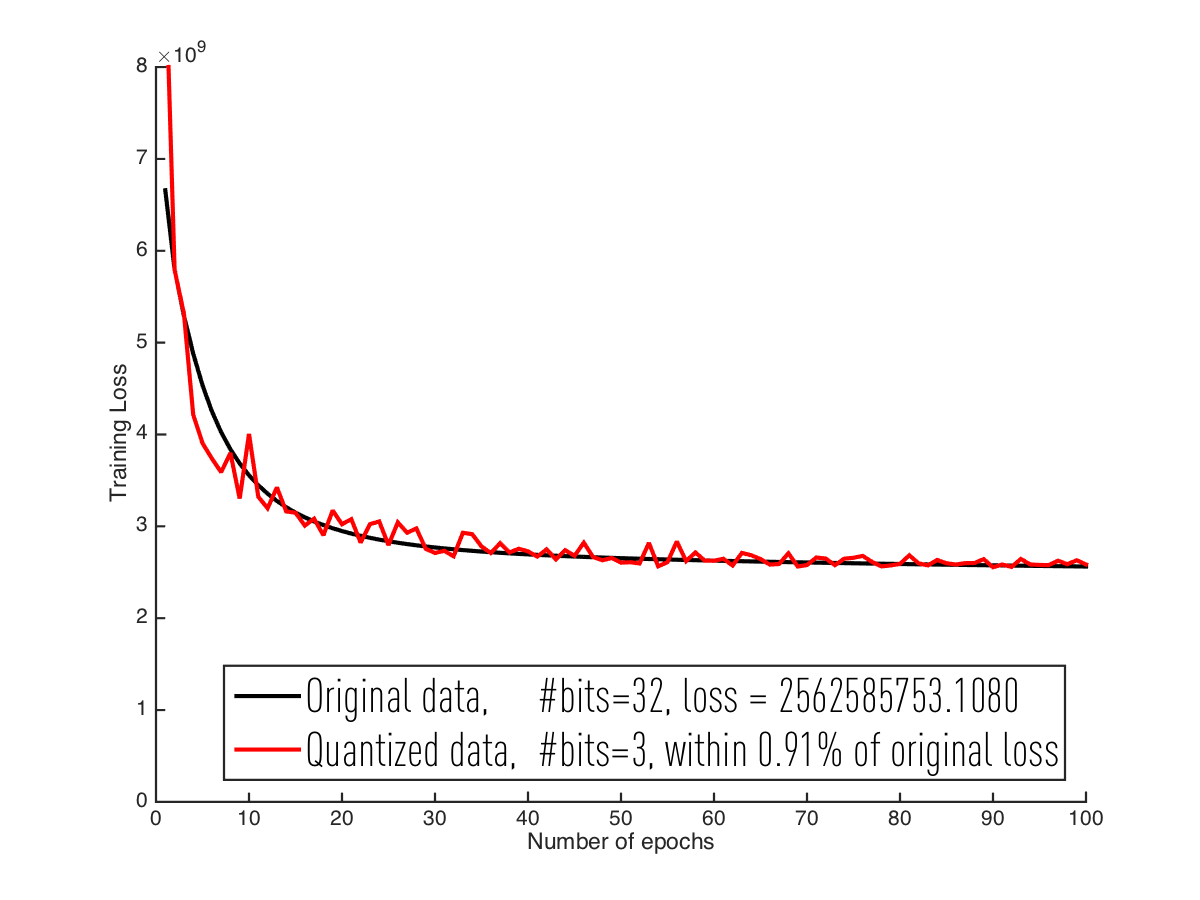
\includegraphics[width=\columnwidth]{lr/real/cadata/d01}
    \caption{Quantized data, initial stepsize = 0.1, 3-bit quantization}
    \end{subfigure}
    \begin{subfigure}[h]{.3\columnwidth}
    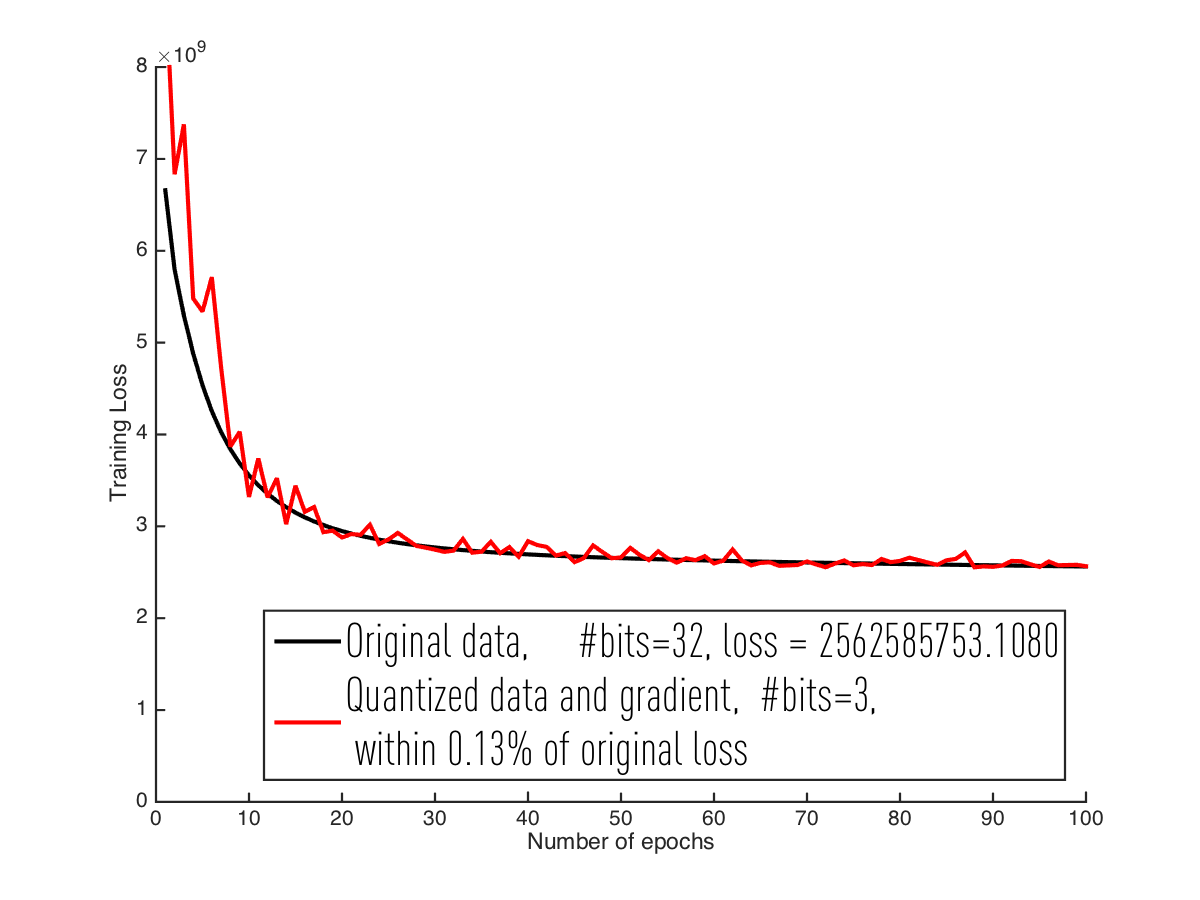
\includegraphics[width=\columnwidth]{lr/real/cadata/dg01}
    \caption{Quantized data and gradient, initial stepsize = 0.1, 3-bit quantization}
    \end{subfigure}
    \begin{subfigure}[h]{.3\columnwidth}
    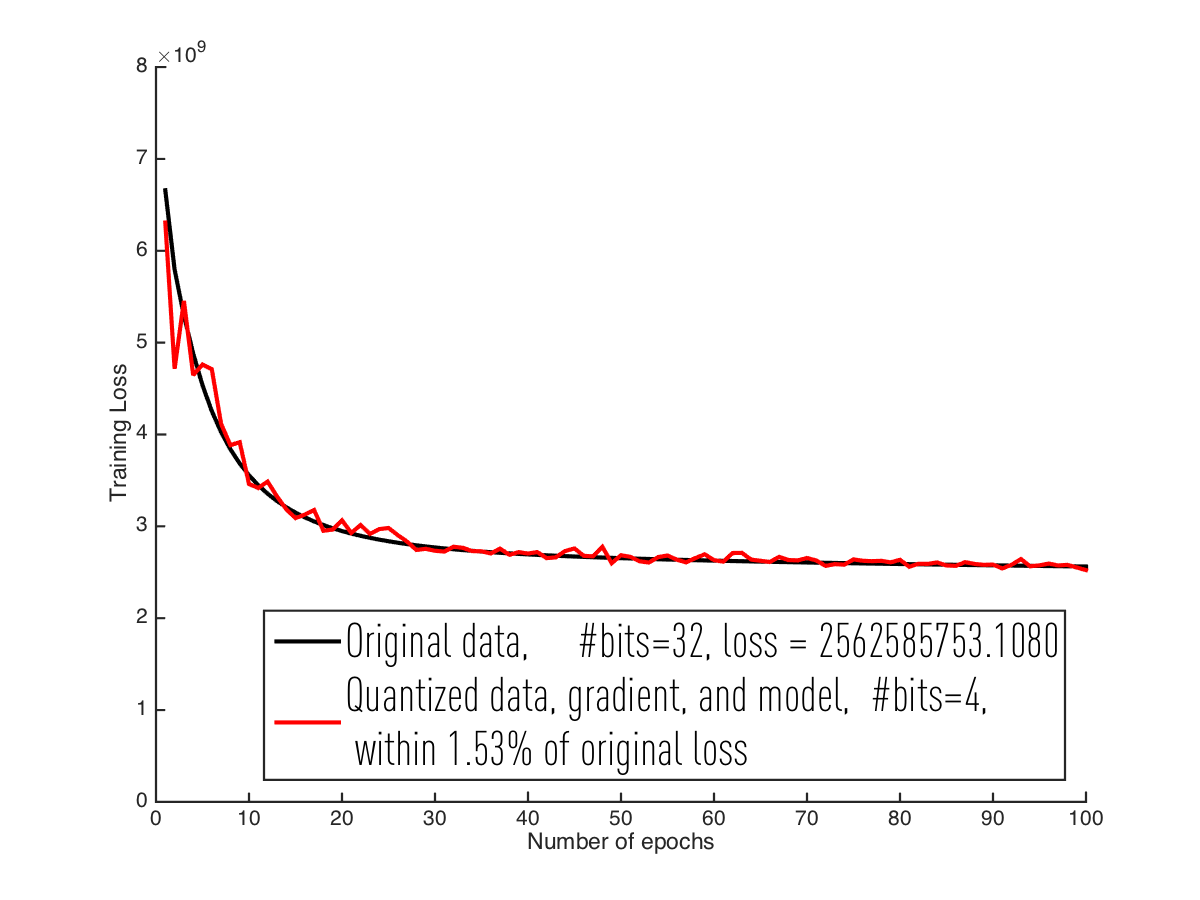
\includegraphics[width=\columnwidth]{lr/real/cadata/dgm01}
     \caption{Quantized data, gradient, and model, initial stepsize = 0.1, 4-bit quantization}
    \end{subfigure}
    
    \begin{subfigure}[h]{.3\columnwidth}
    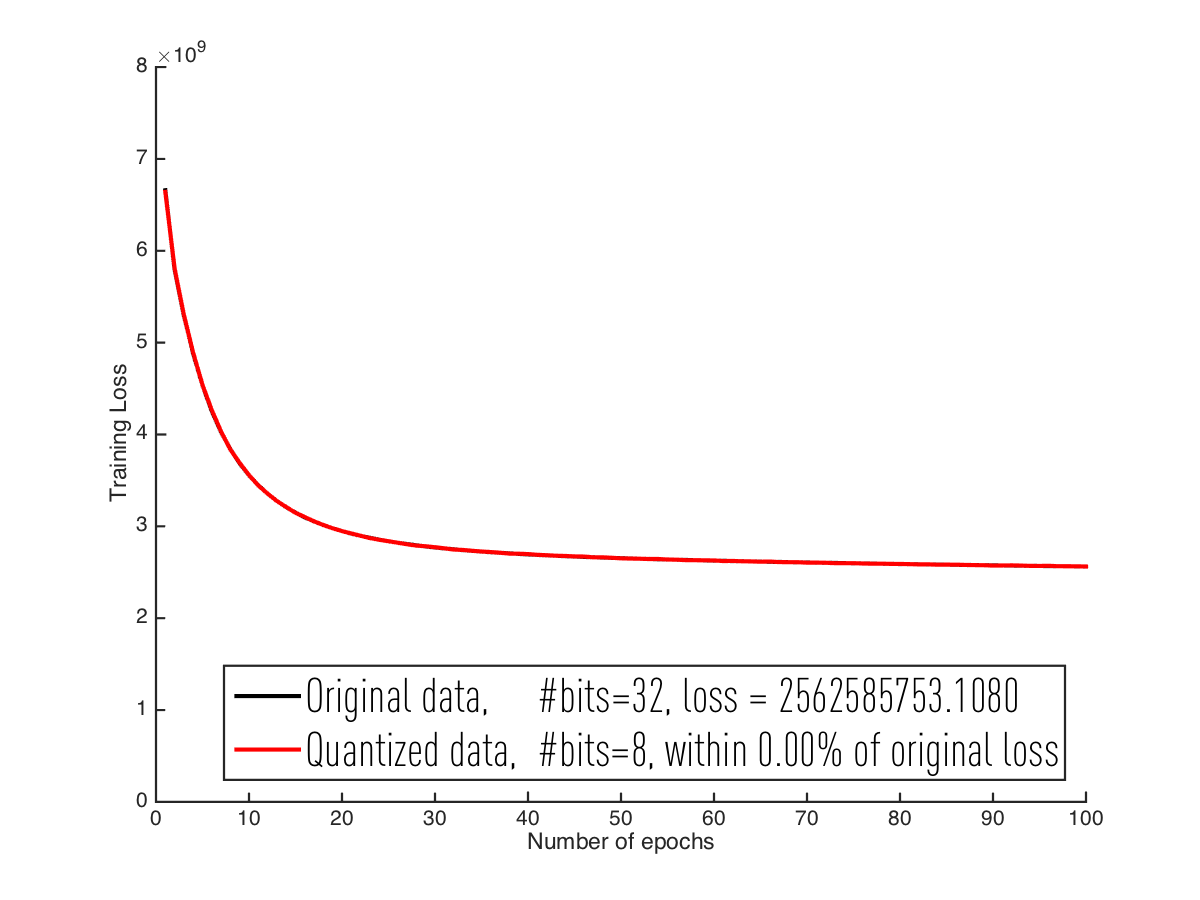
\includegraphics[width=\columnwidth]{lr/real/cadata/8d01}
    \caption{Quantized data, initial stepsize = 0.1, 8-bit quantization}
    \end{subfigure}
    \begin{subfigure}[h]{.3\columnwidth}
    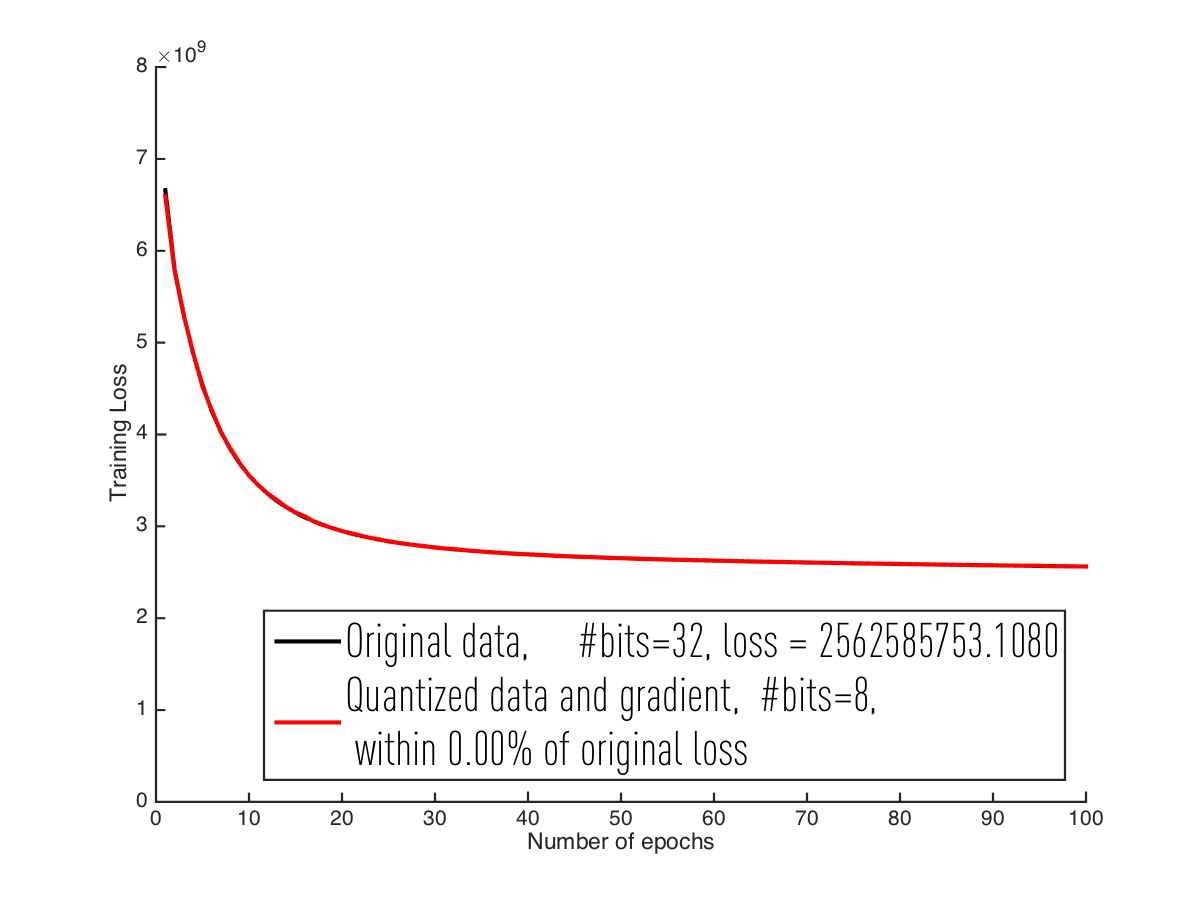
\includegraphics[width=\columnwidth]{lr/real/cadata/8dg01}
    \caption{Quantized data and gradient, initial stepsize = 0.1, 8-bit quantization}
    \end{subfigure}
    \begin{subfigure}[h]{.3\columnwidth}
    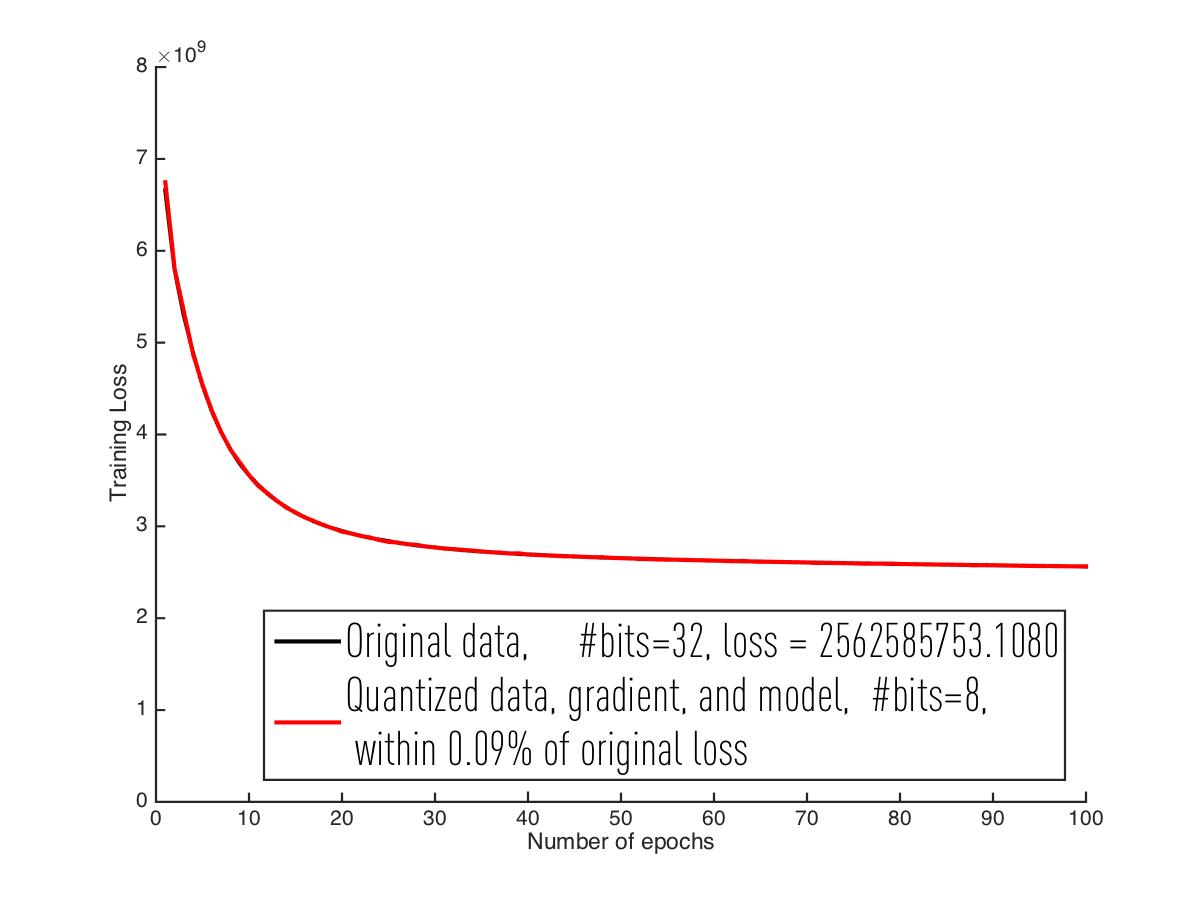
\includegraphics[width=\columnwidth]{lr/real/cadata/8dgm01}
     \caption{Quantized data, gradient, and model, initial stepsize = 0.1, 8-bit quantization}
    \end{subfigure}
    
\caption{ZipML on Linear Regression using \texttt{cadata} dataset. 3-bit version is good enough to get a comparable empirical convergence rate to the same loss; with 8-bit we get almost the same result as the original 32-bit data}
\label{fig:lrcadata}
\end{figure}


\begin{figure}[h]
\centering
   
    \begin{subfigure}[h]{.3\columnwidth}
    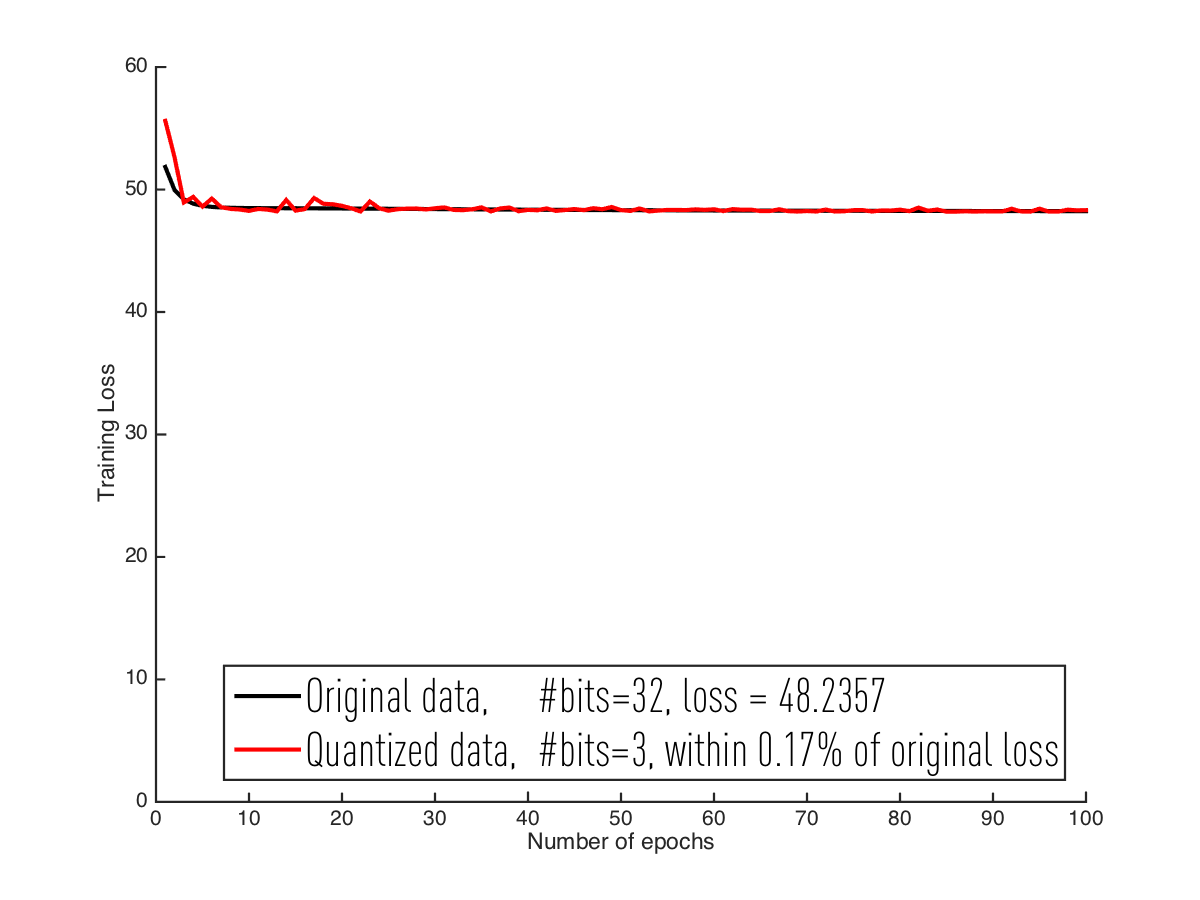
\includegraphics[width=\columnwidth]{lr/real/cpusmall/d01}
    \caption{Quantized data, initial stepsize = 0.1}
    \end{subfigure}
    \begin{subfigure}[h]{.3\columnwidth}
    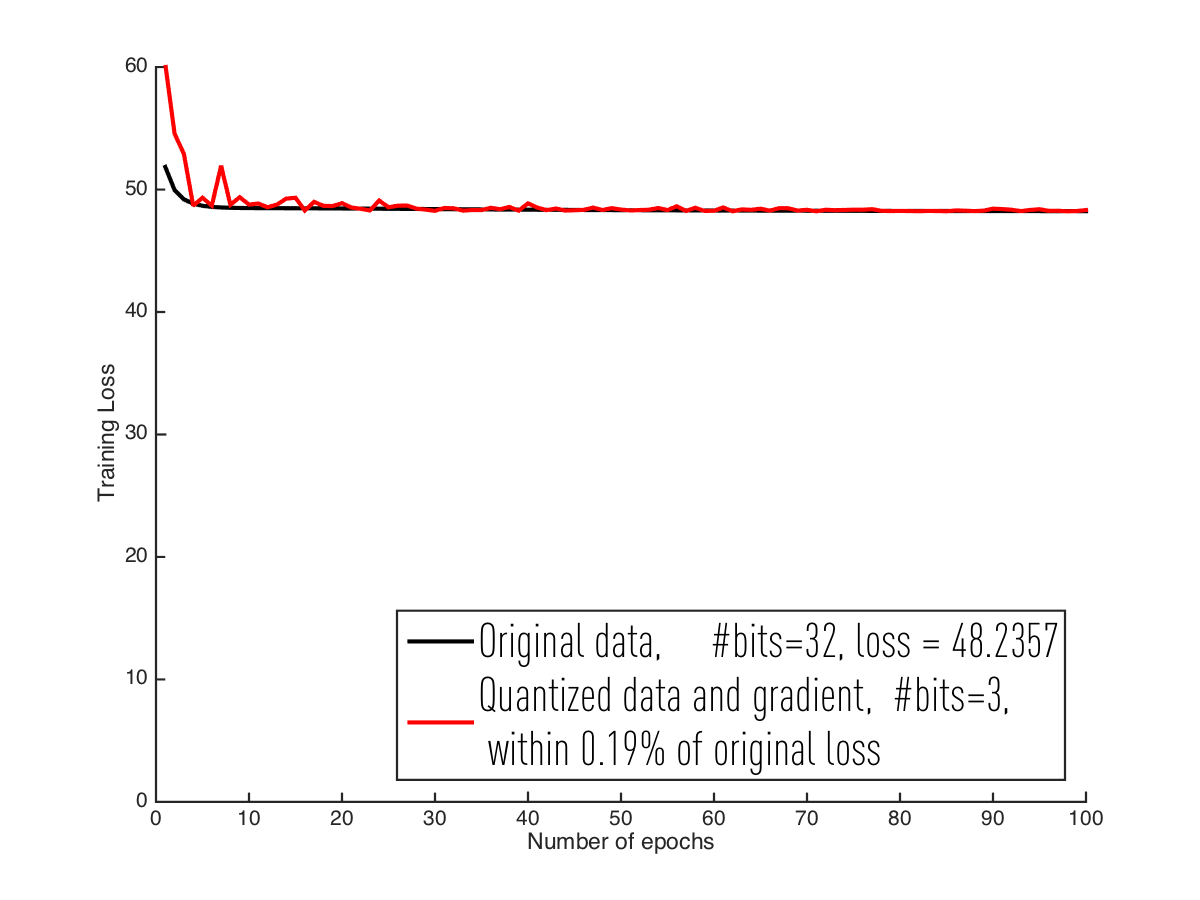
\includegraphics[width=\columnwidth]{lr/real/cpusmall/dg01}
    \caption{Quantized data and gradient, initial stepsize = 0.1}
    \end{subfigure}
    \begin{subfigure}[h]{.3\columnwidth}
    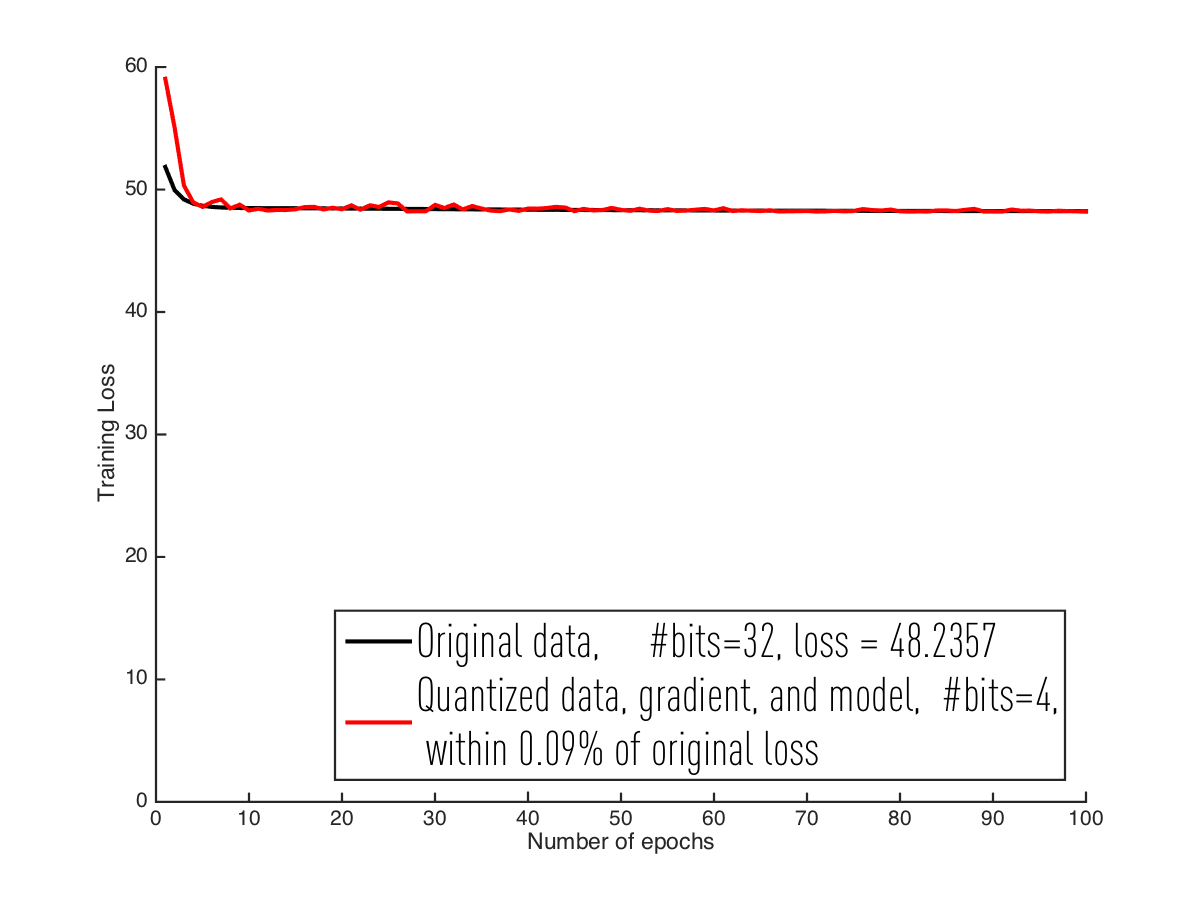
\includegraphics[width=\columnwidth]{lr/real/cpusmall/dgm01}
     \caption{Quantized data, gradient, and model, initial stepsize = 0.1}
    \end{subfigure}
    
\caption{ZipML on Linear Regression using \texttt{cpusmall} dataset}
\label{fig:lrcpusmall}
\end{figure}

\begin{figure}[h]
\centering
 
    \begin{subfigure}[h]{.3\columnwidth}
    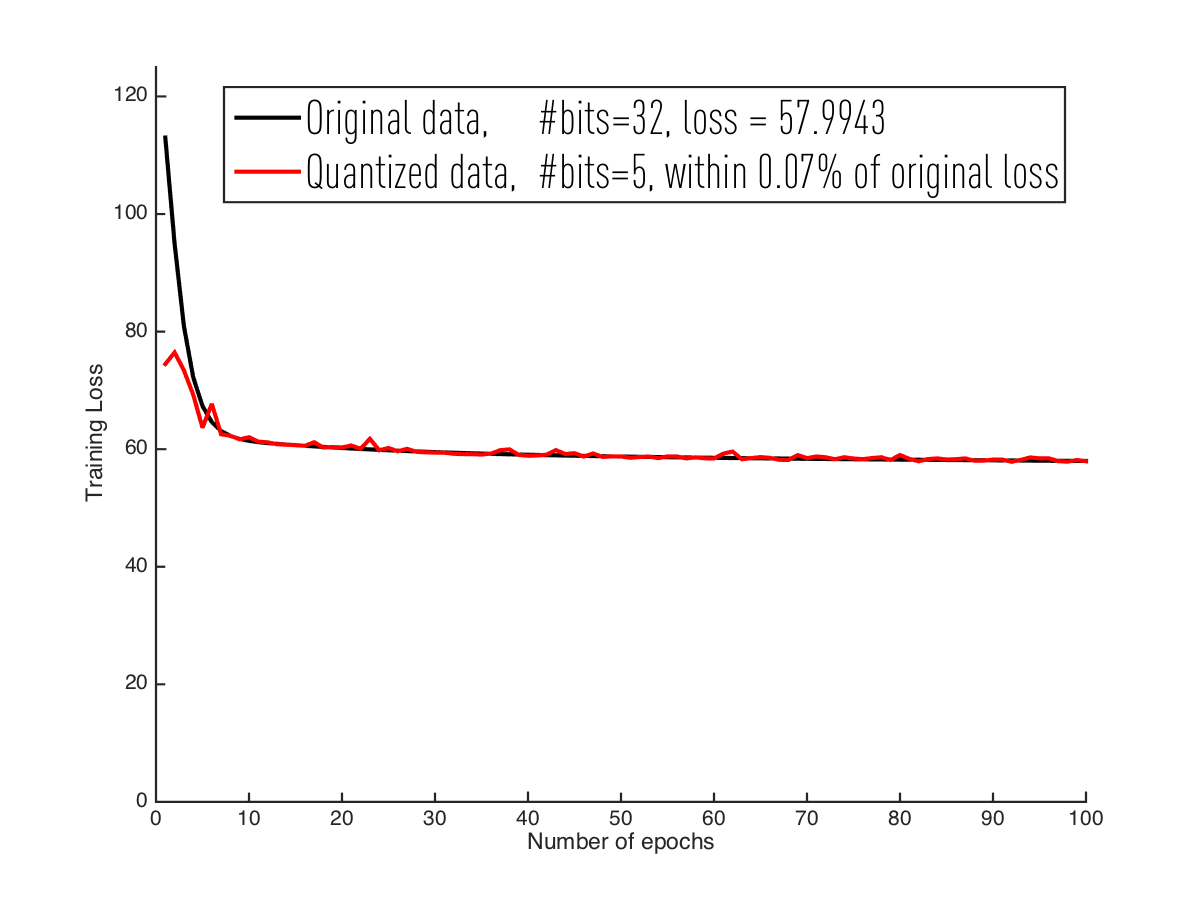
\includegraphics[width=\columnwidth]{lr/real/YearPredictionMSD/d001}
    \caption{Quantized data, initial stepsize = 0.01}
    \end{subfigure}
    \begin{subfigure}[h]{.3\columnwidth}
    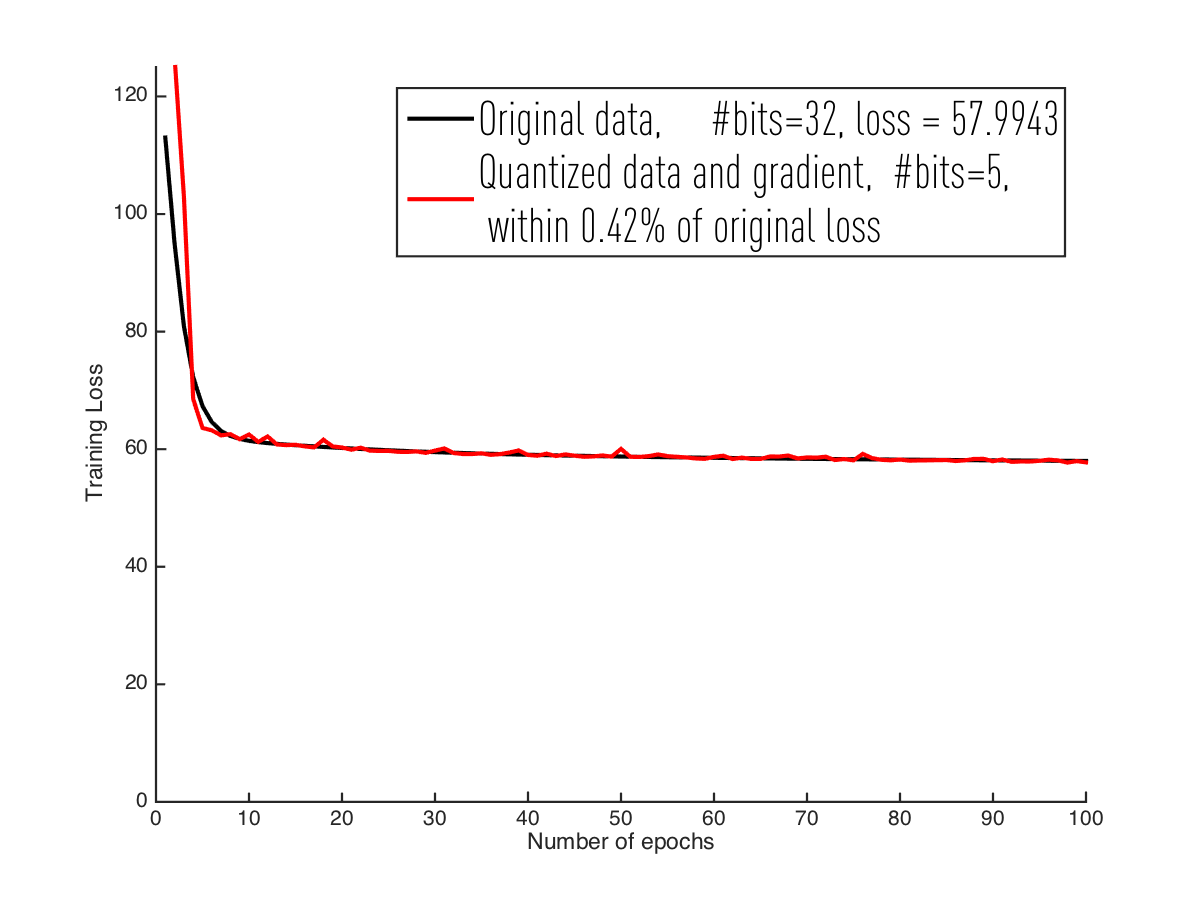
\includegraphics[width=\columnwidth]{lr/real/YearPredictionMSD/dg001}
    \caption{Quantized data and gradient, initial stepsize = 0.01}
    \end{subfigure}
    \begin{subfigure}[h]{.3\columnwidth}
    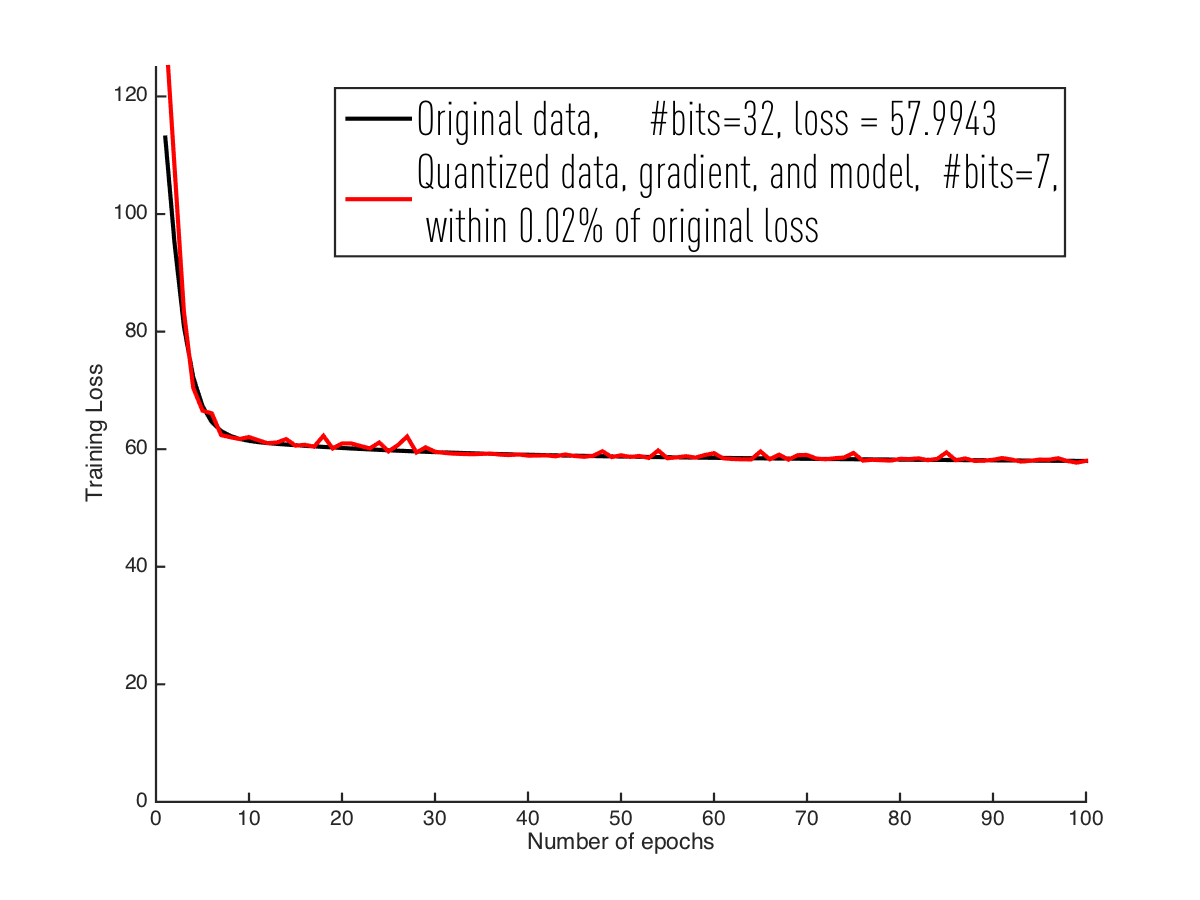
\includegraphics[width=\columnwidth]{lr/real/YearPredictionMSD/dgm001}
     \caption{Quantized data, gradient, and model, initial stepsize = 0.01}
     \label{subfig:musicdgm}
    \end{subfigure}
    
\caption{ZipML on Linear Regression using \texttt{music} dataset}
\label{fig:lrmusic}
\end{figure}

\begin{figure}[h]
\centering
    \begin{subfigure}[h]{.3\columnwidth}
    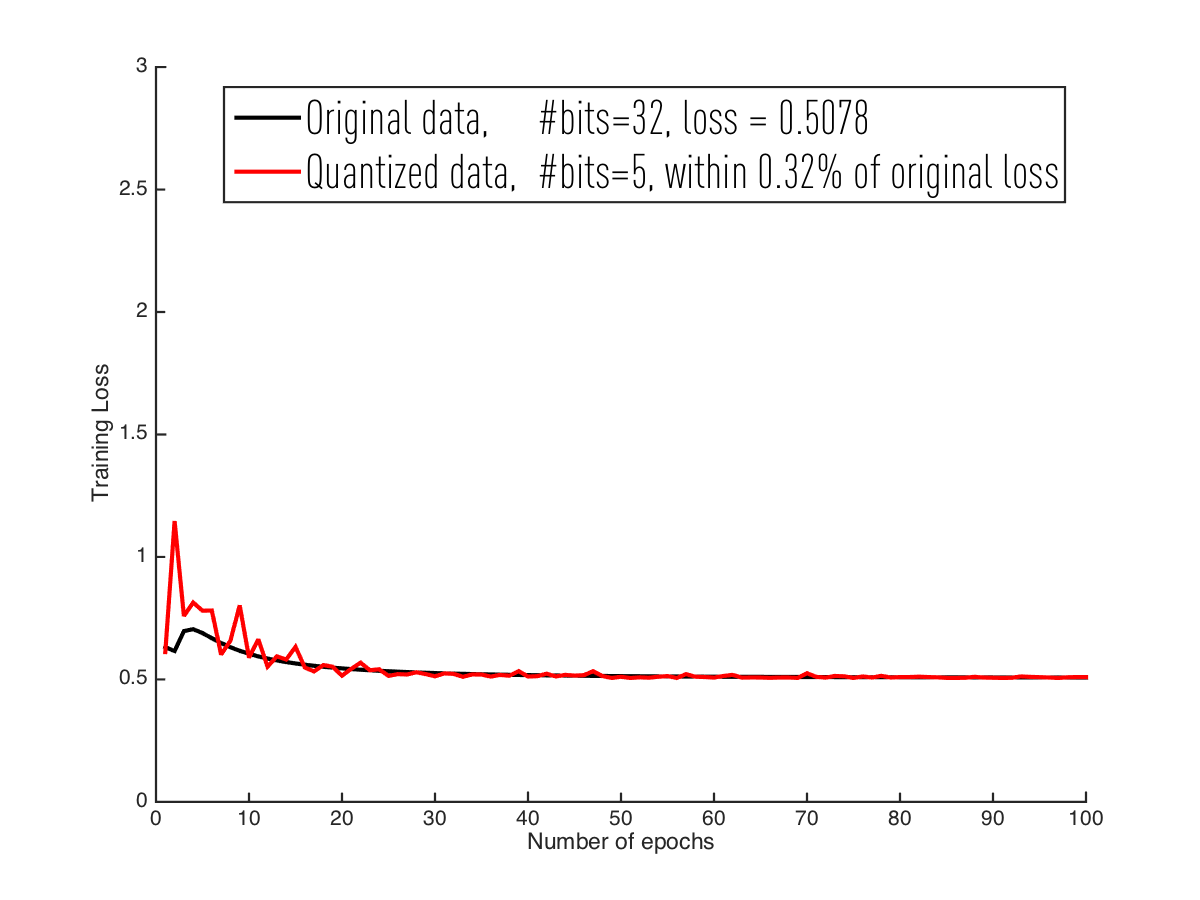
\includegraphics[width=\columnwidth]{lr/synthetic/20easy/d01}
    \caption{Quantized data, initial stepsize = 0.1}
    \end{subfigure}
    \begin{subfigure}[h]{.3\columnwidth}
    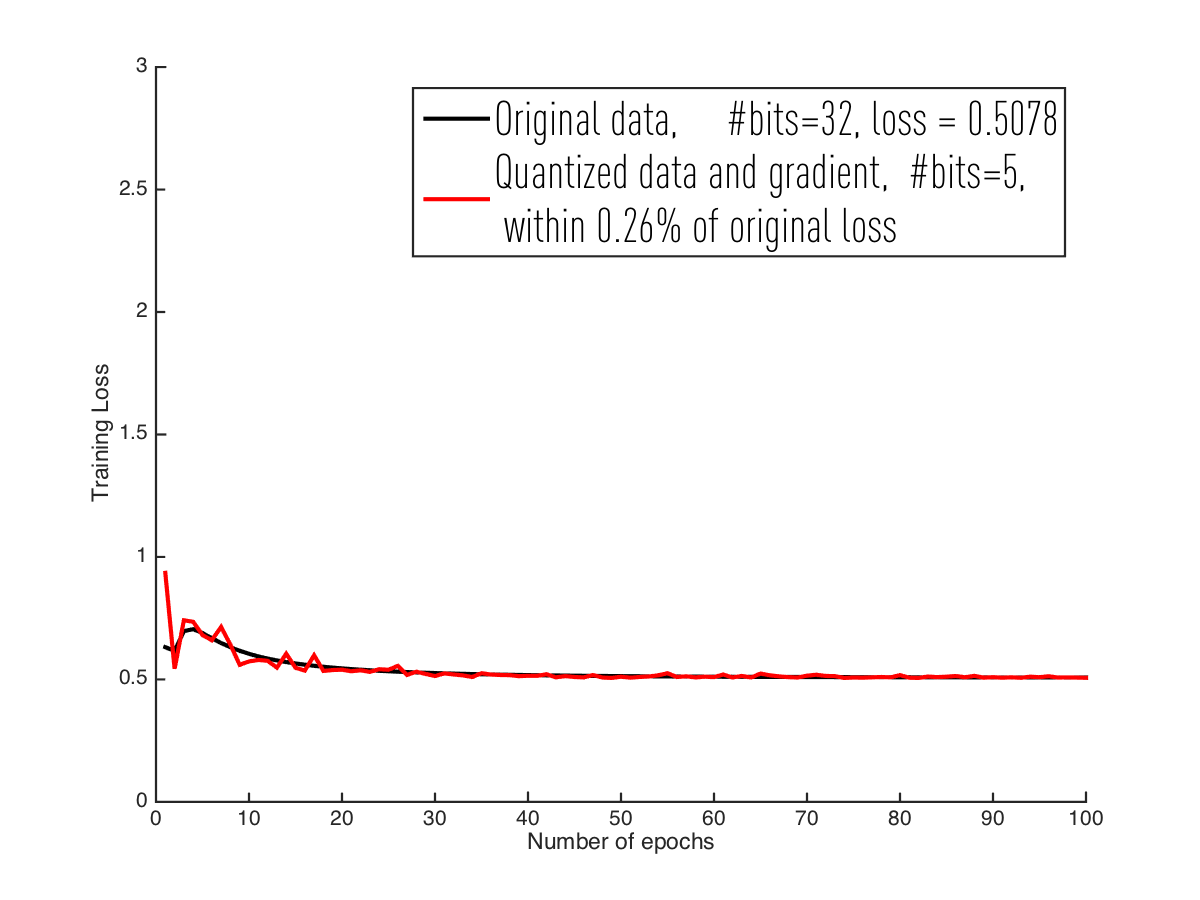
\includegraphics[width=\columnwidth]{lr/synthetic/20easy/dg01}
    \caption{Quantized data and gradient, initial stepsize = 0.1}
    \end{subfigure}
    \begin{subfigure}[h]{.3\columnwidth}
    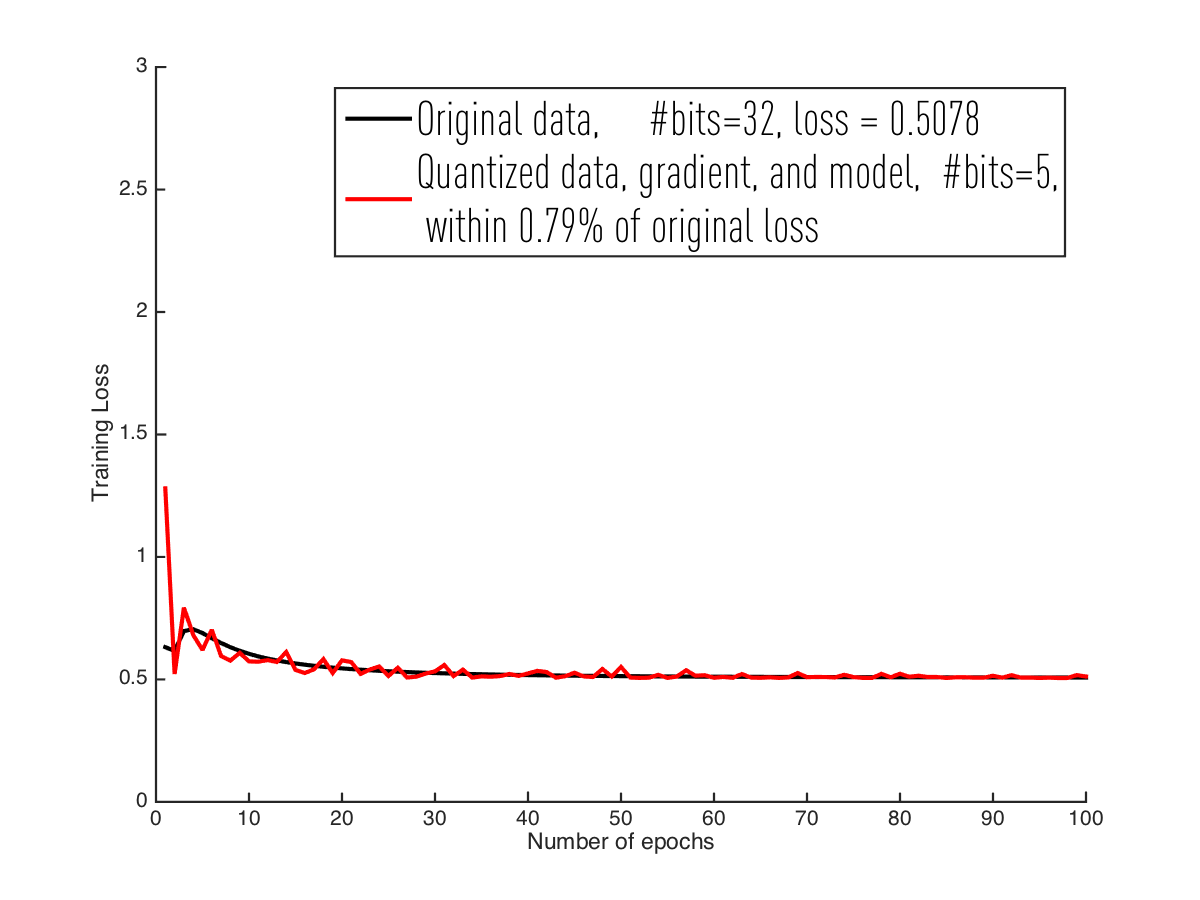
\includegraphics[width=\columnwidth]{lr/synthetic/20easy/dgm01}
     \caption{Quantized data, gradient, and model, initial stepsize = 0.1}
    \end{subfigure}
    
\caption{ZipML on Linear Regression using \texttt{synthetic} dataset with 20 features and standard deviation 1}
\label{fig:lr20easy}
\end{figure}

\begin{figure}[h]
\centering
    \begin{subfigure}[h]{.3\columnwidth}
    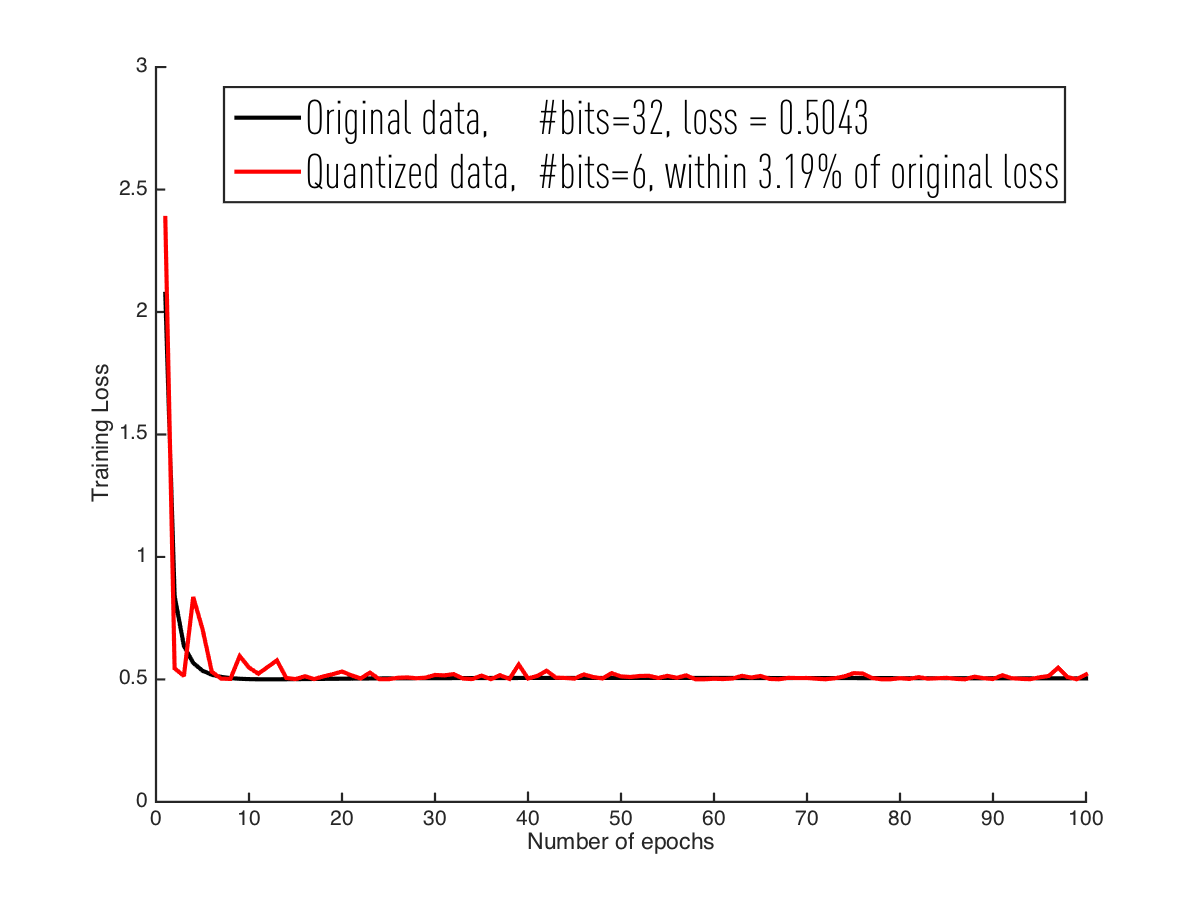
\includegraphics[width=\columnwidth]{lr/synthetic/20hard/d01}
    \caption{Quantized data, initial stepsize = 0.1}
    \end{subfigure}
    \begin{subfigure}[h]{.3\columnwidth}
    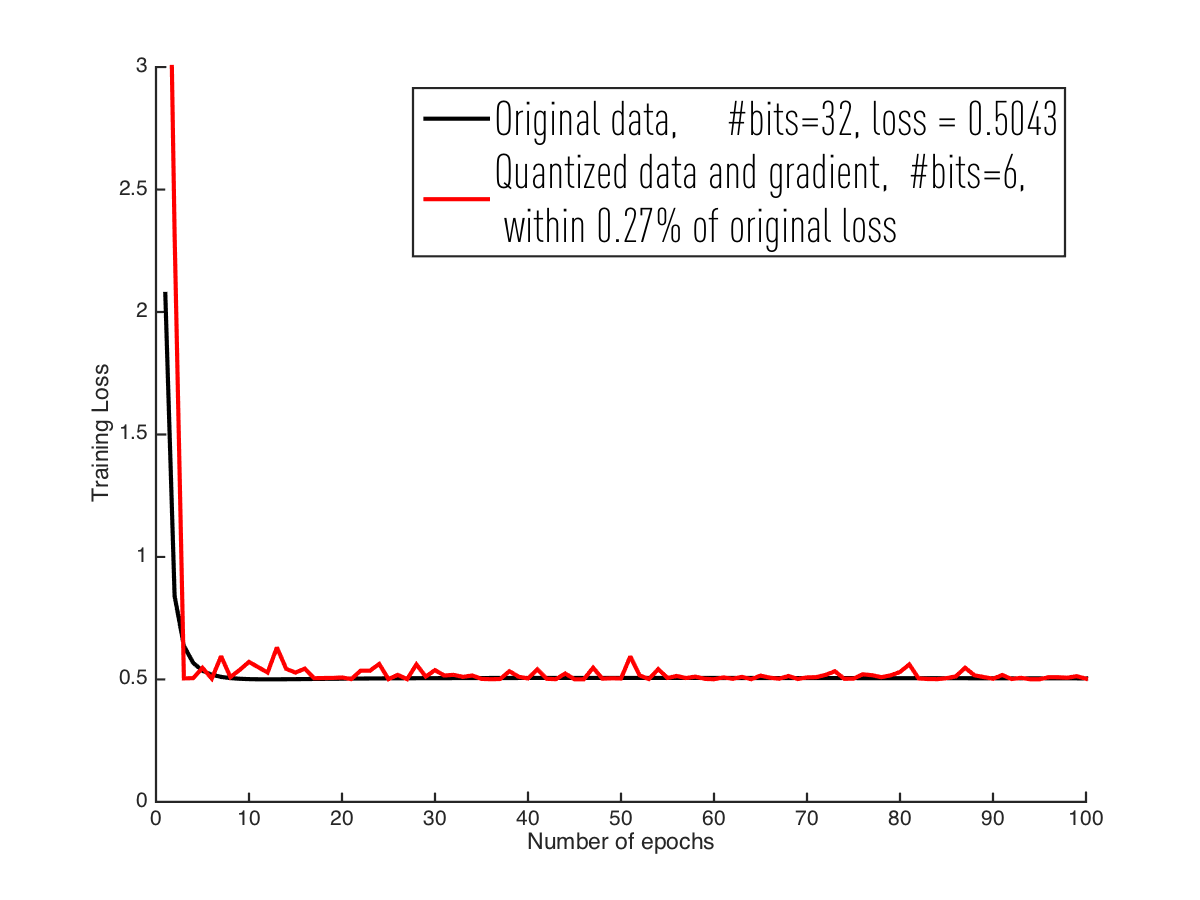
\includegraphics[width=\columnwidth]{lr/synthetic/20hard/dg01}
    \caption{Quantized data and gradient, initial stepsize = 0.1}
    \end{subfigure}
    \begin{subfigure}[h]{.3\columnwidth}
    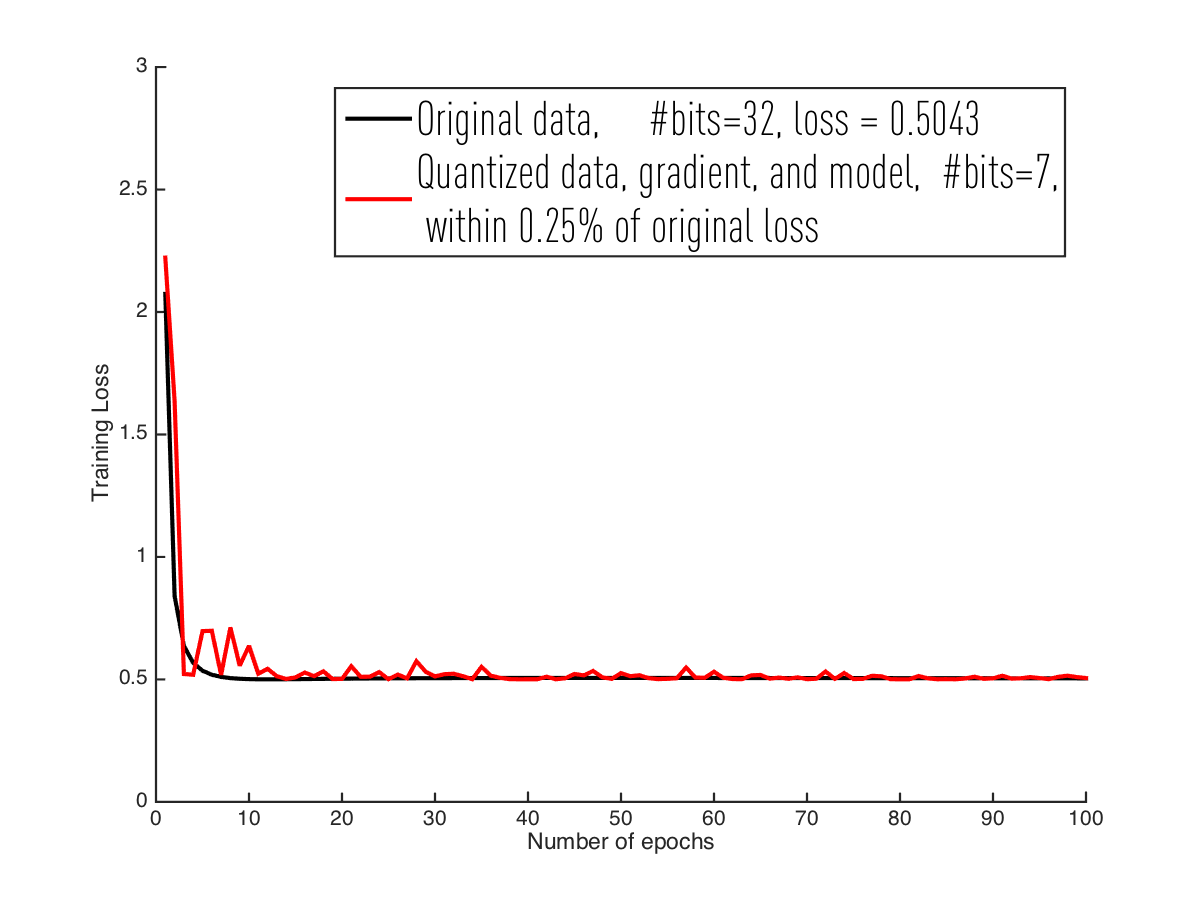
\includegraphics[width=\columnwidth]{lr/synthetic/20hard/dgm01}
     \caption{Quantized data, gradient, and model, initial stepsize = 0.1}
    \end{subfigure}
    
\caption{ZipML on Linear Regression using \texttt{synthetic} dataset with 20 features and standard deviation 4}
\label{fig:lr20hard}
\end{figure}

\begin{figure}[h]
\centering
   
    \begin{subfigure}[h]{.3\columnwidth}
    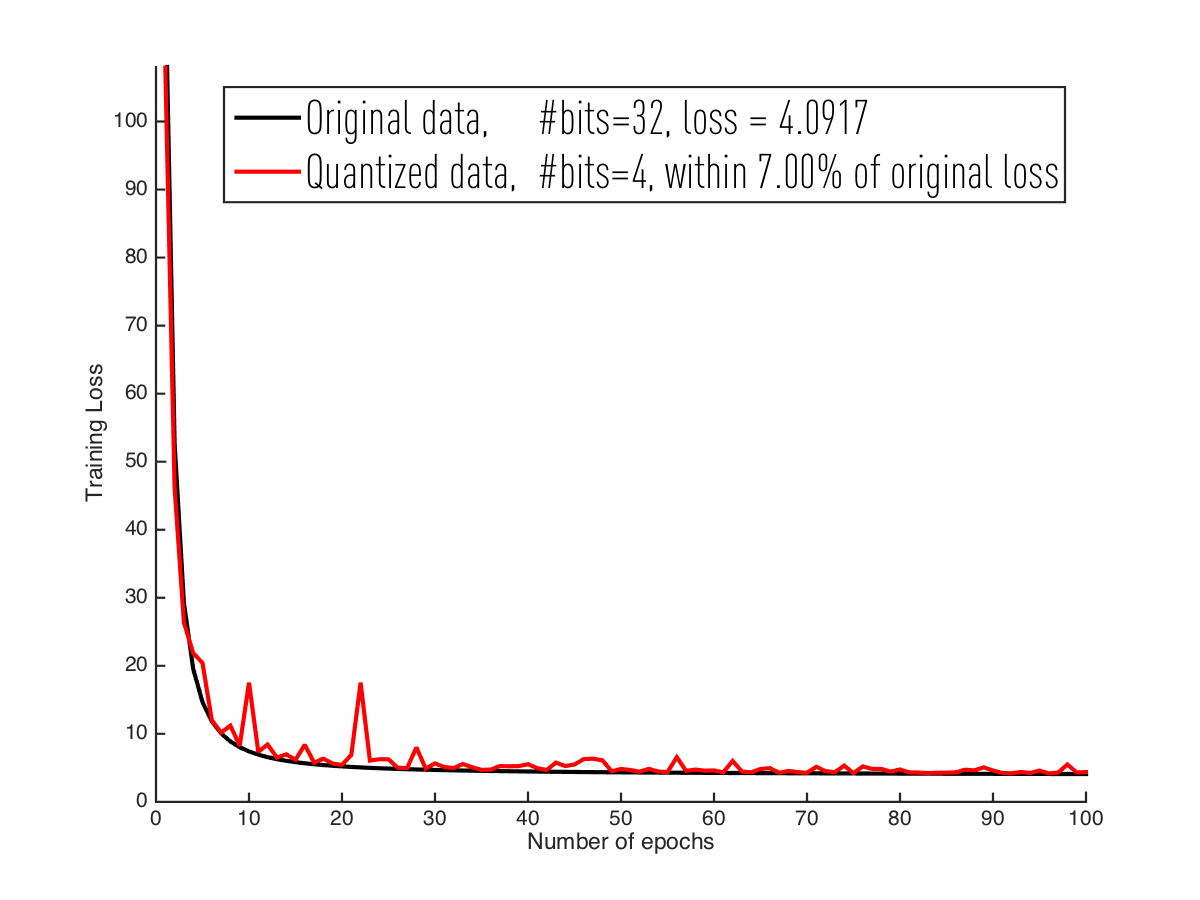
\includegraphics[width=\columnwidth]{lr/synthetic/160hard/d001}
    \caption{Quantized data, initial stepsize = 0.01}
    \end{subfigure}
    \begin{subfigure}[h]{.3\columnwidth}
    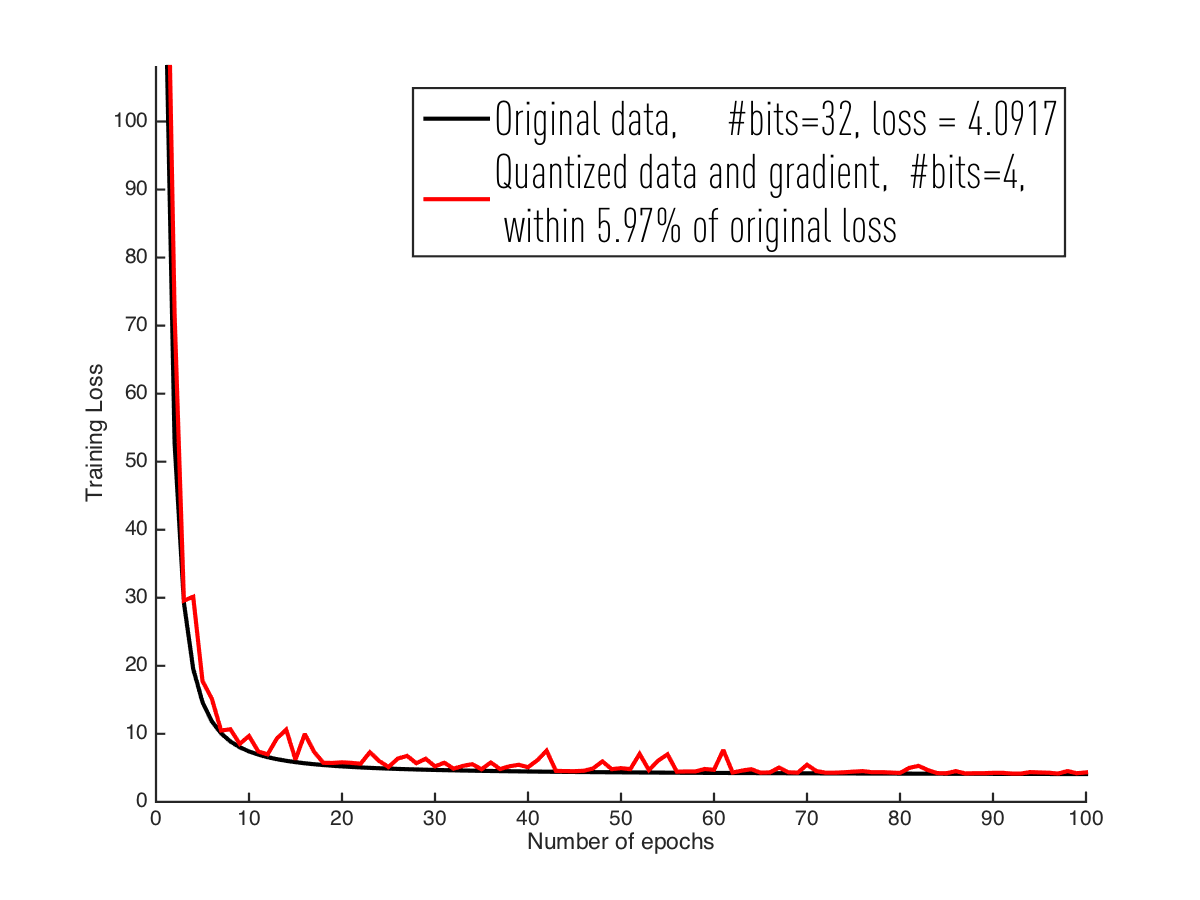
\includegraphics[width=\columnwidth]{lr/synthetic/160hard/dg001}
    \caption{Quantized data and gradient, initial stepsize = 0.01}
    \end{subfigure}
    \begin{subfigure}[h]{.3\columnwidth}
    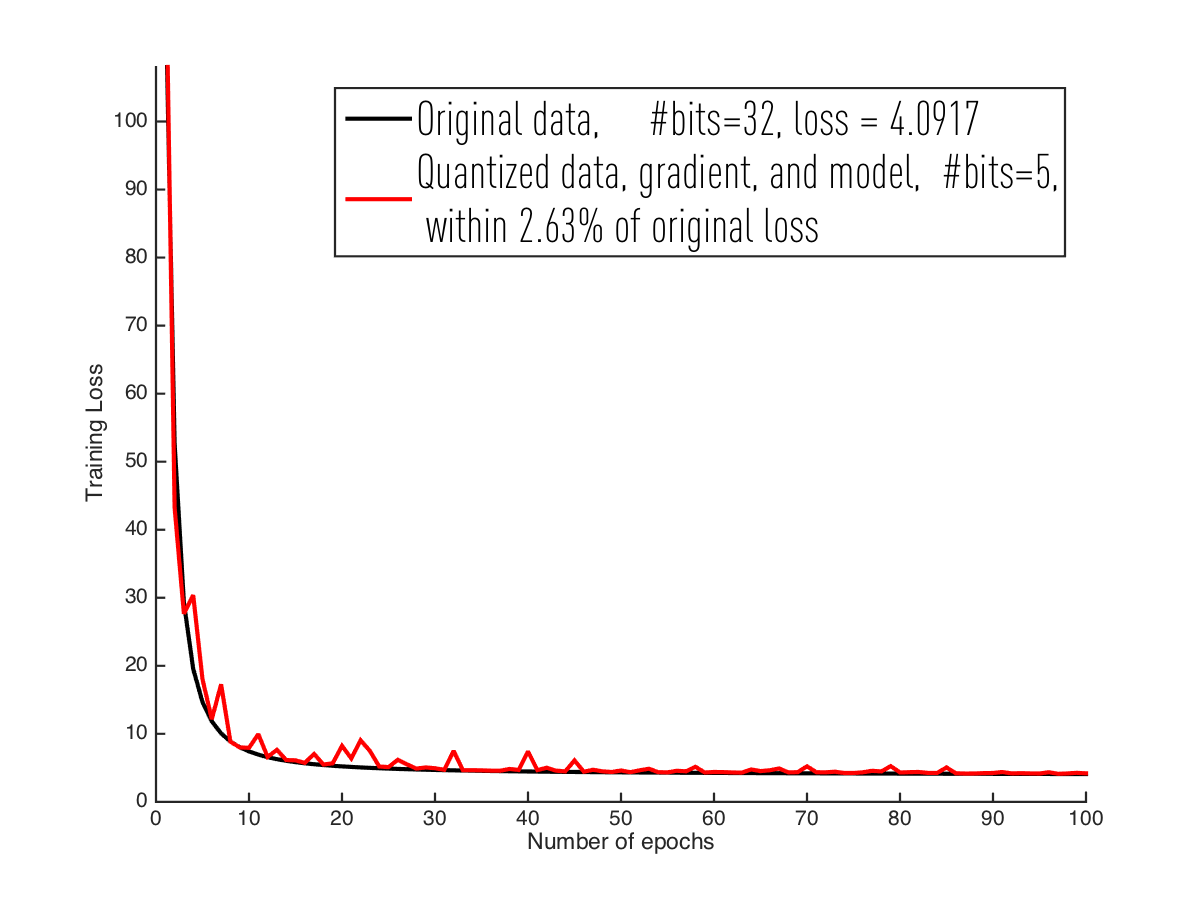
\includegraphics[width=\columnwidth]{lr/synthetic/160hard/dgm001}
     \caption{Quantized data, gradient, and model, initial stepsize = 0.01}
    \end{subfigure}
    
\caption{ZipML on Linear Regression using \texttt{synthetic} dataset with 160 features and standard deviation 4}
\label{fig:lr160hard}
\end{figure}




\subsection{Least Squares Support Vector Machines}

We now validate ZipML for least squares SVM.
We present the results for \texttt{cod-rna} in Figure~\ref{fig:lssvmcodrna}, the result for \texttt{covtype} in Figure~\ref{fig:lssvmcovtype}, and the result for \texttt{ijcnn} in Figure~\ref{fig:lssvmijcnn},

Figures~\ref{fig:lssvmcodrna}-\ref{fig:lssvmijcnn} illustrate that for all datasets we choose and all stepsizes we run, our quantization framework
converges to the same solution with comparable
empirical convergence rate and that 3-bit quantization is sufficient to achieve that.


\begin{figure}[h]
\centering
    \begin{subfigure}[h]{.3\columnwidth}
    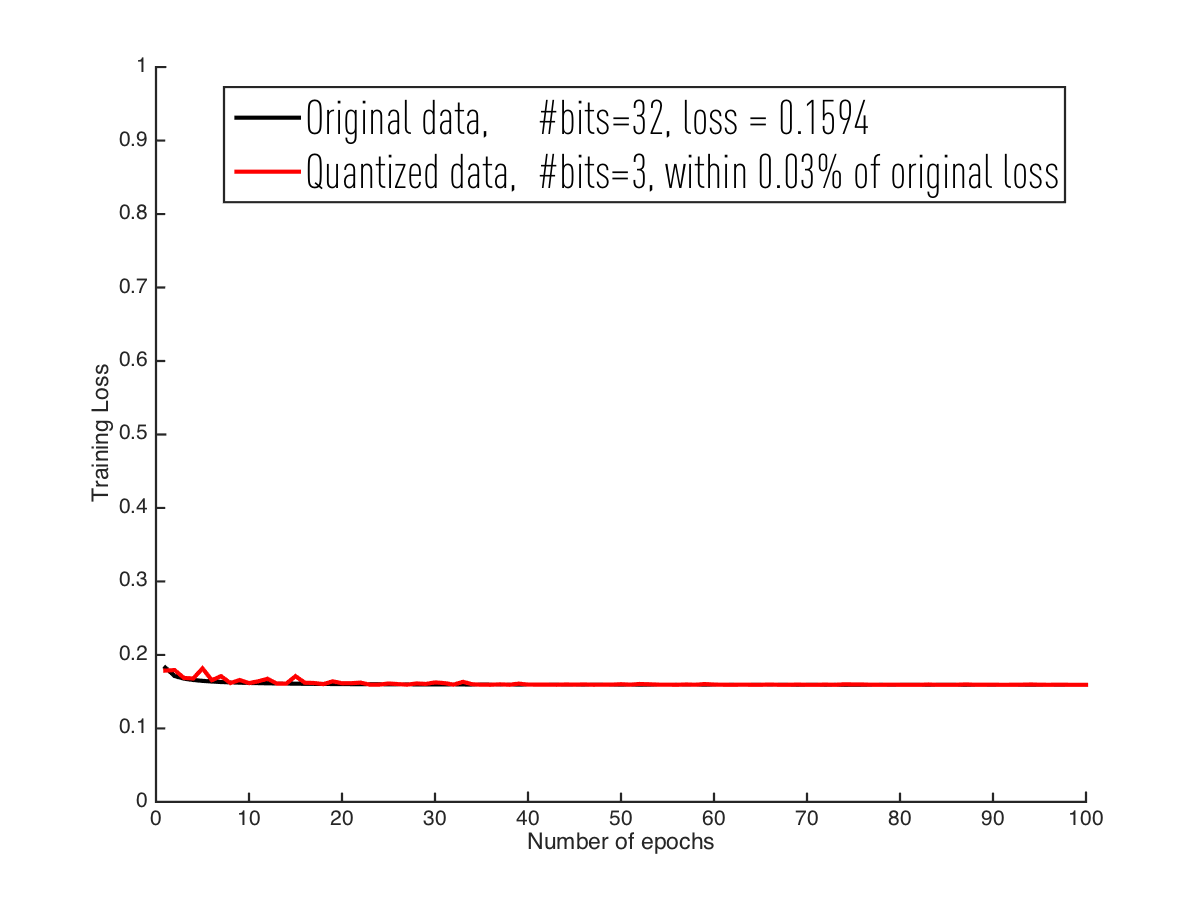
\includegraphics[width=\columnwidth]{lssvm/cod-rna/d001}
    \caption{Quantized data, initial stepsize = 0.01}
    \end{subfigure}
    \begin{subfigure}[h]{.3\columnwidth}
    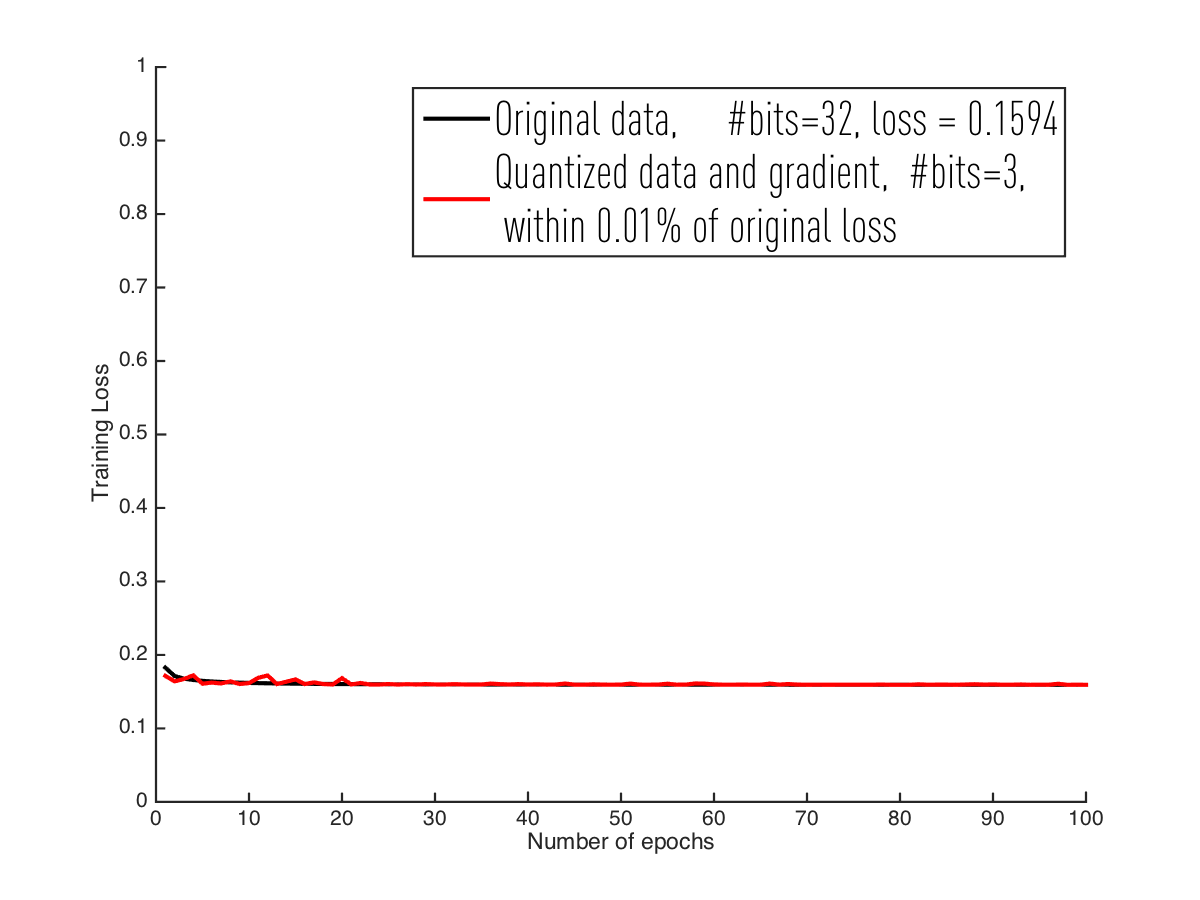
\includegraphics[width=\columnwidth]{lssvm/cod-rna/dg001}
    \caption{Quantized data and gradient, initial stepsize = 0.01}
    \end{subfigure}
    \begin{subfigure}[h]{.3\columnwidth}
    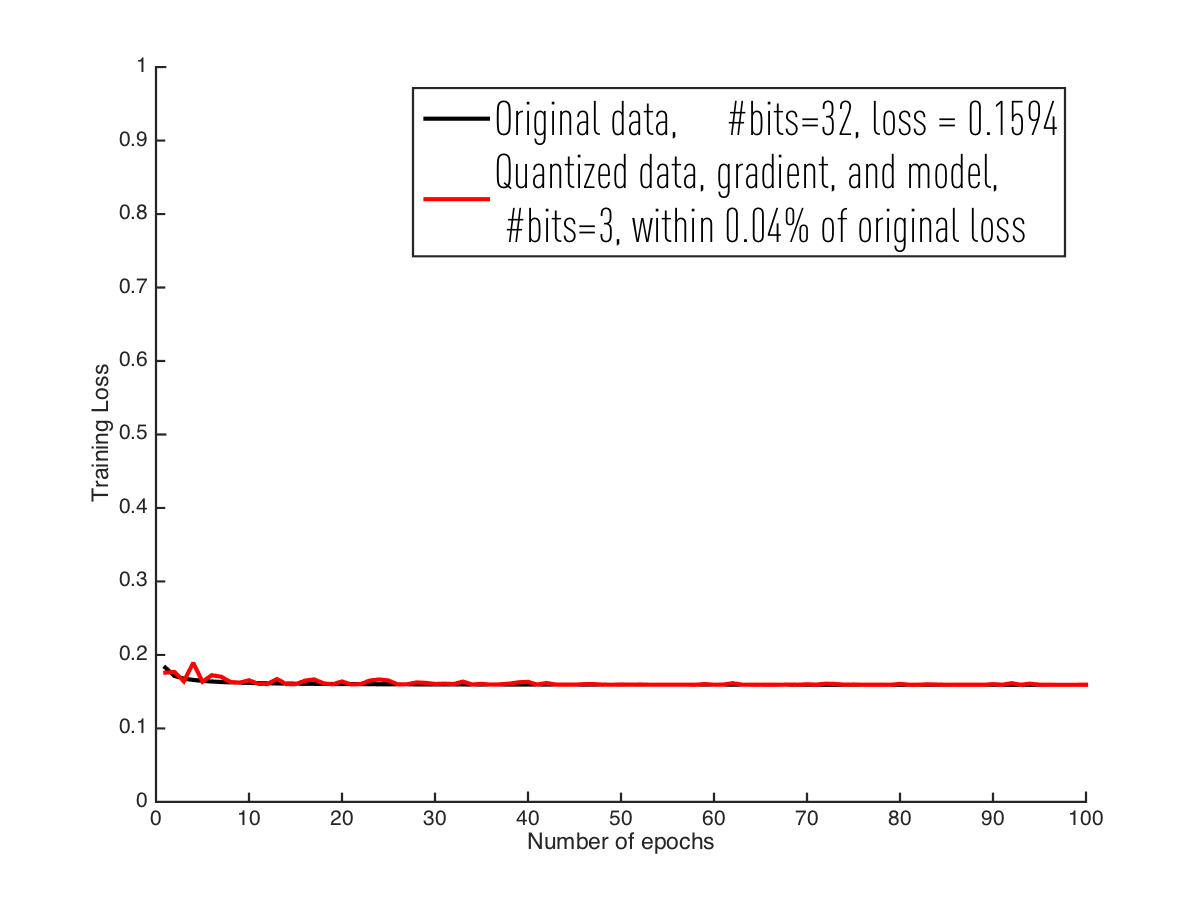
\includegraphics[width=\columnwidth]{lssvm/cod-rna/dgm001}
     \caption{Quantized data, gradient, and model, initial stepsize = 0.01}
    \end{subfigure}
    
\caption{ZipML on LSSVM using \texttt{cod-rna} dataset}
\label{fig:lssvmcodrna}
\end{figure}

\begin{figure}[h]
\centering
    \begin{subfigure}[h]{.3\columnwidth}
    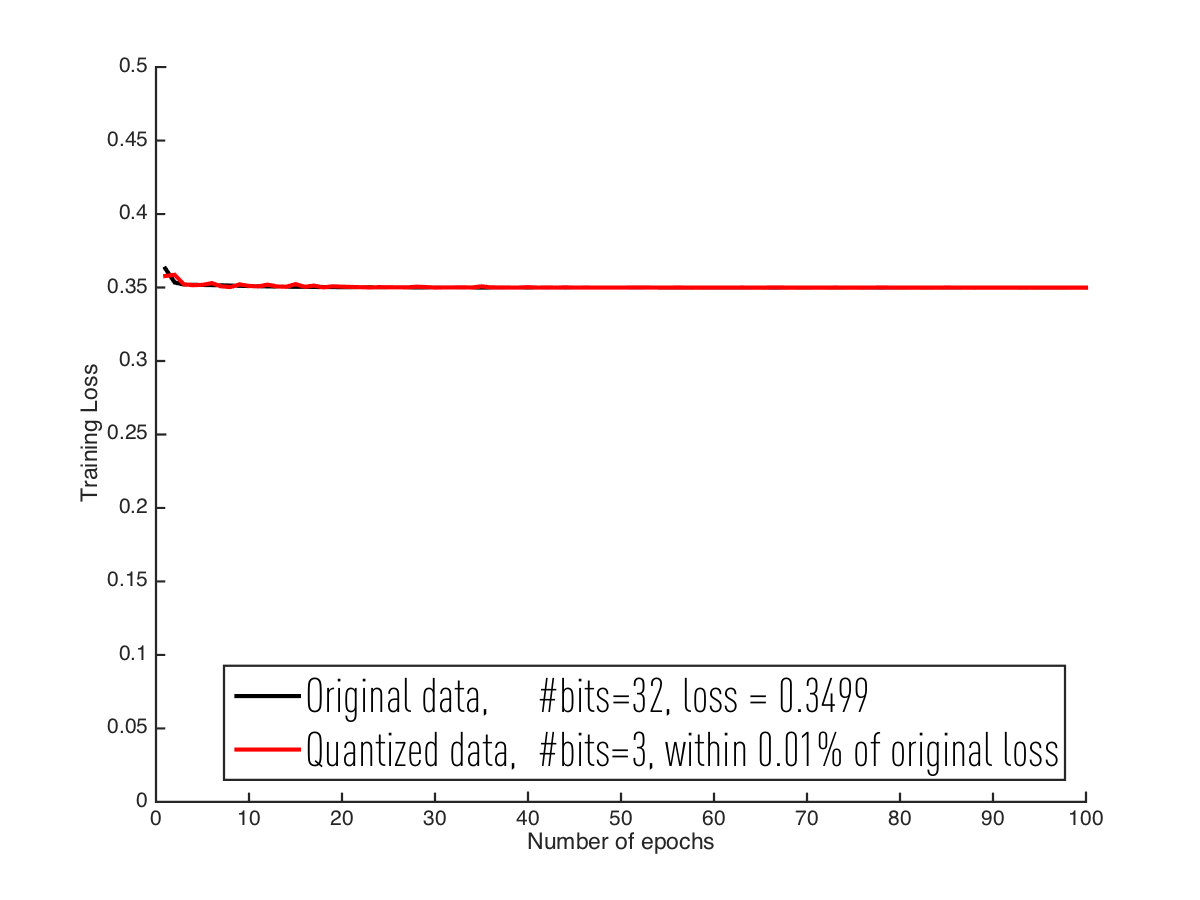
\includegraphics[width=\columnwidth]{lssvm/cov-type/d001}
    \caption{Quantized data, initial stepsize = 0.01}
    \end{subfigure}
    \begin{subfigure}[h]{.3\columnwidth}
    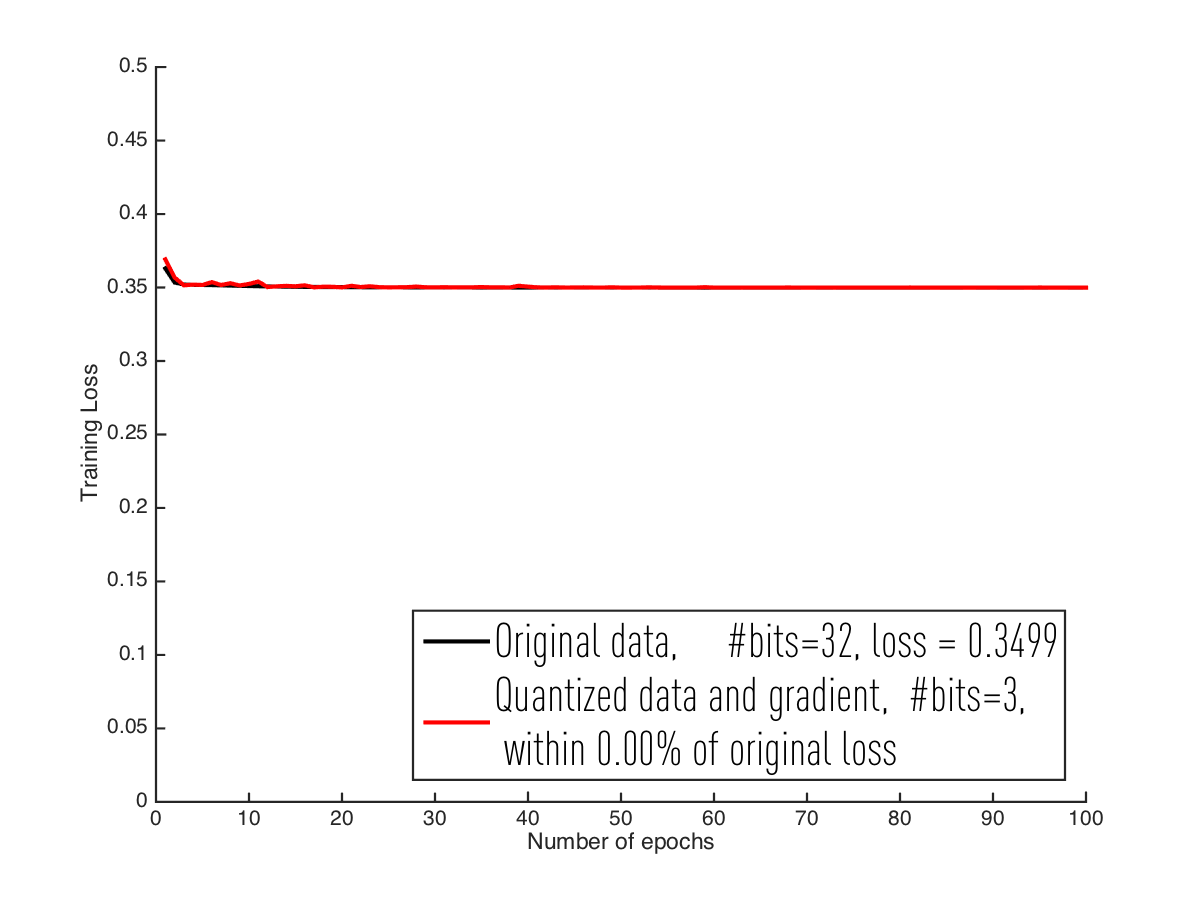
\includegraphics[width=\columnwidth]{lssvm/cov-type/dg001}
    \caption{Quantized data and gradient, initial stepsize = 0.01}
    \end{subfigure}
    \begin{subfigure}[h]{.3\columnwidth}
    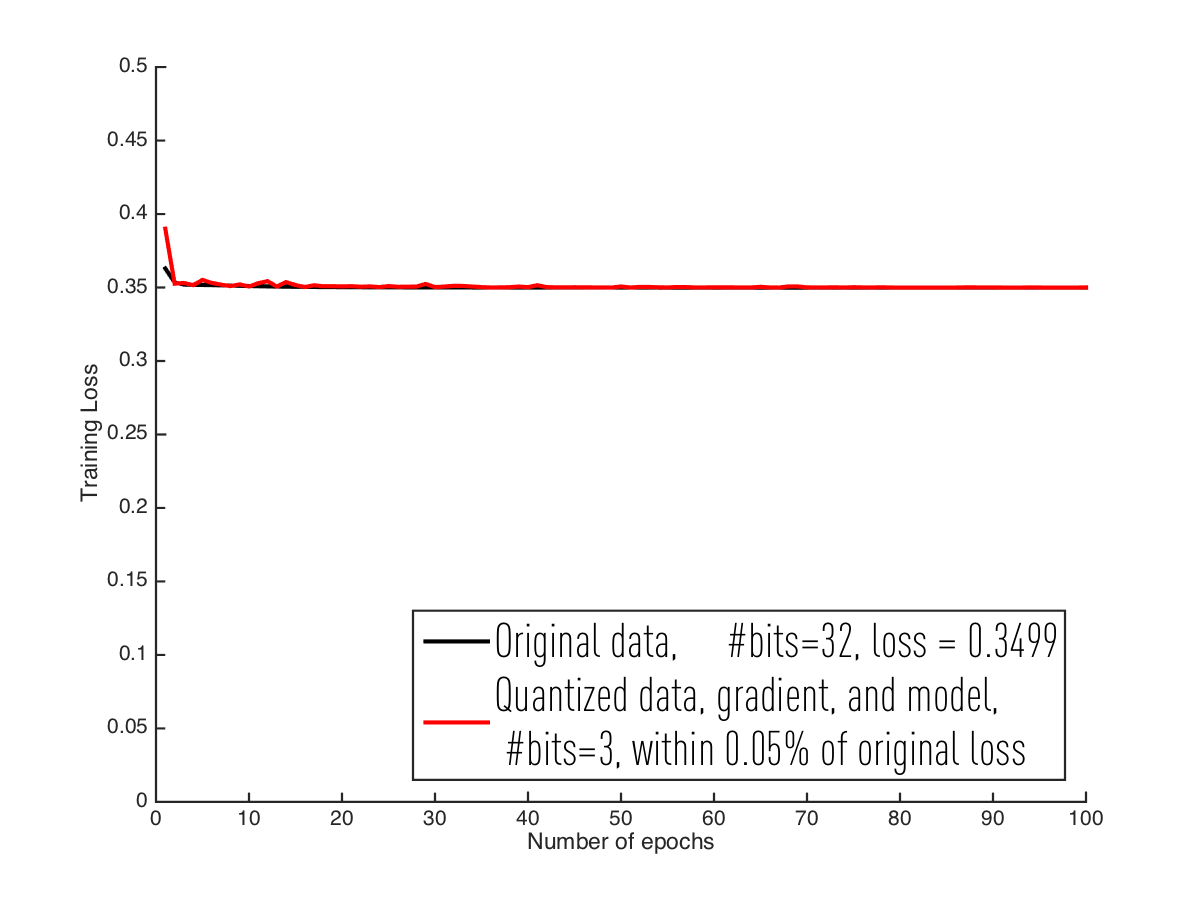
\includegraphics[width=\columnwidth]{lssvm/cov-type/dgm001}
     \caption{Quantized data, gradient, and model, initial stepsize = 0.01}
    \end{subfigure}
    
\caption{ZipML on LSSVM using \texttt{covtype} dataset}
\label{fig:lssvmcovtype}
\end{figure}



\begin{figure}[h]
\centering
    \begin{subfigure}[h]{.3\columnwidth}
    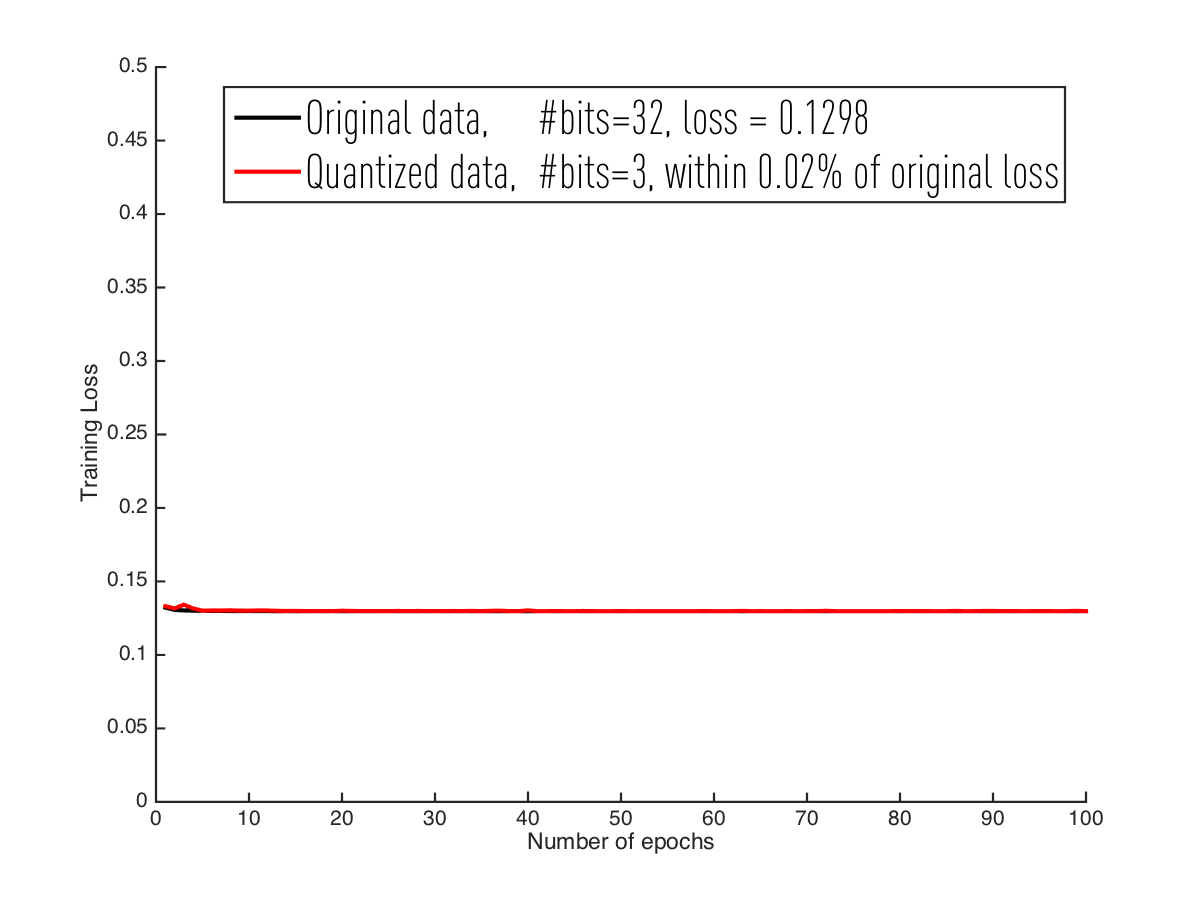
\includegraphics[width=\columnwidth]{lssvm/ijcnn/d001}
    \caption{Quantized data, initial stepsize = 0.01}
    \end{subfigure}
    \begin{subfigure}[h]{.3\columnwidth}
    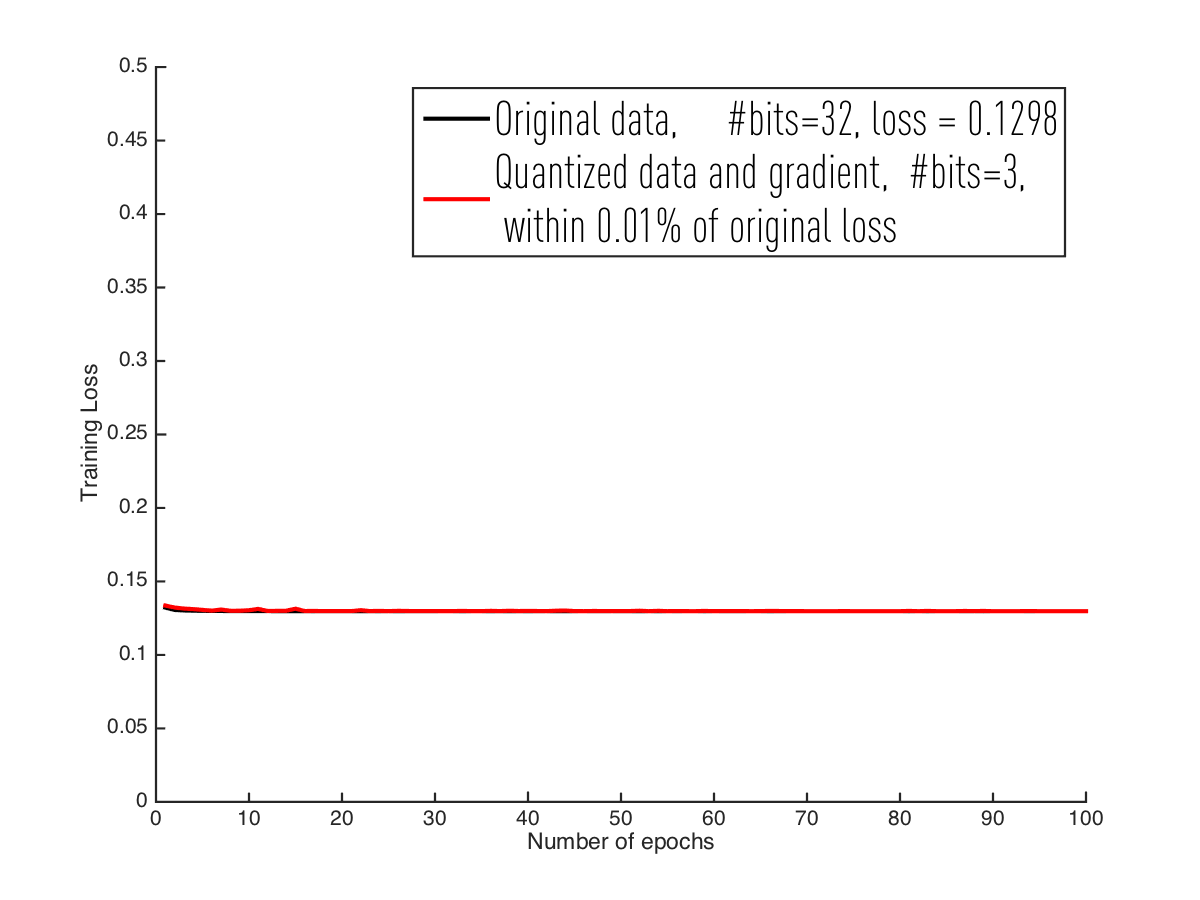
\includegraphics[width=\columnwidth]{lssvm/ijcnn/dg001}
    \caption{Quantized data and gradient, initial stepsize = 0.01}
    \end{subfigure}
    \begin{subfigure}[h]{.3\columnwidth}
    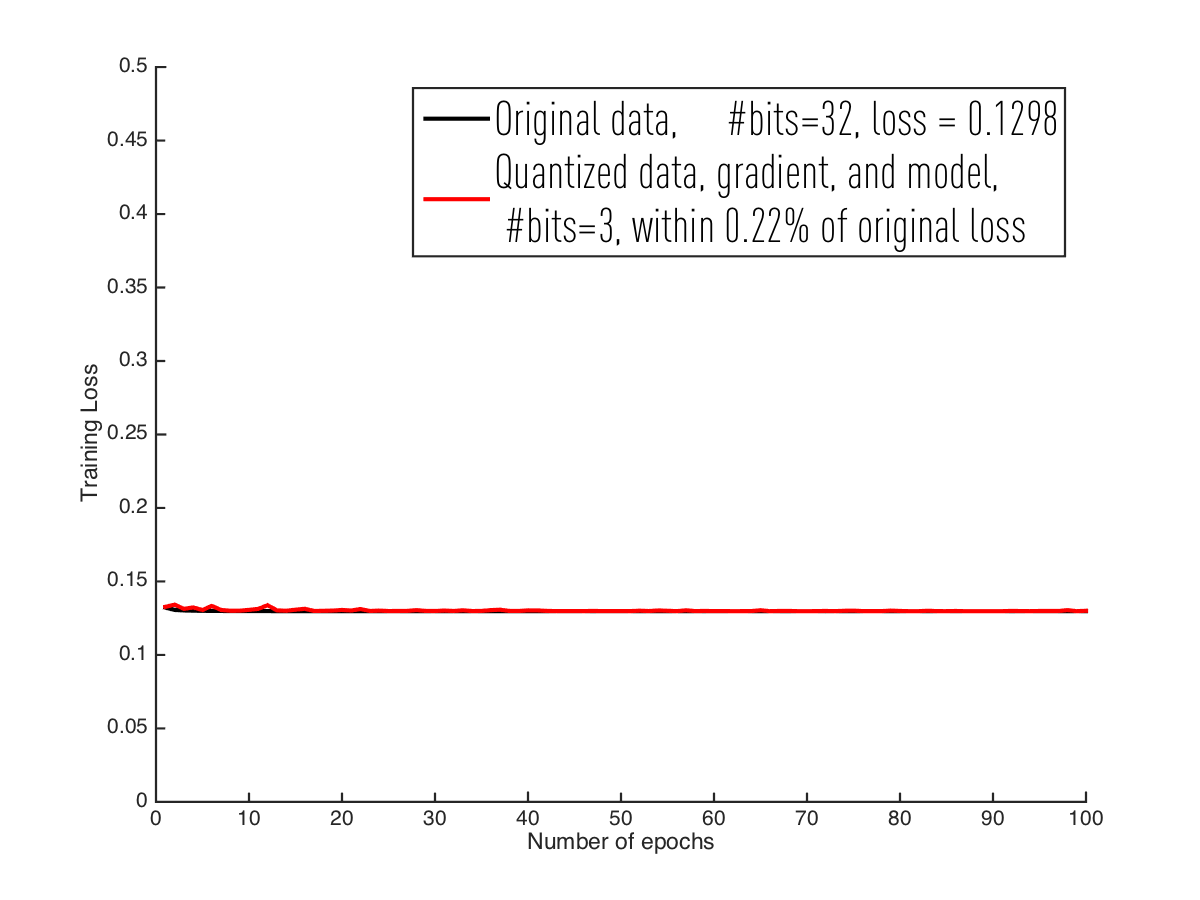
\includegraphics[width=\columnwidth]{lssvm/ijcnn/dgm001}
     \caption{Quantized data, gradient, and model, initial stepsize = 0.01}
    \end{subfigure}
    
\caption{ZipML on LSSVM using \texttt{ijcnn} dataset}
\label{fig:lssvmijcnn}
\end{figure}



\subsection{Support Vector Machines}
\label{sec:svm}

Finally we validate ZipML in the context of support vector machines (SVM).

Our experimental results for SVM are given in Figure~\ref{fig:svm}. For all datasets and stepsizes we chose, 8-bit quantization was good enough to converge to the same solution with using original data. By using importance sampling, we only need to fetch 32-bit orginal data 2\% to 7\% times. This will add an overhead of at most 2.34 bits on average for each sample we quantize, meaning that each sample we quantize is on average about 10-bit. We get comparable results to running SVM with original data, while using 3 times less memory.%\todo{Over what?}

\begin{figure}[h]
\centering
    \begin{subfigure}[b]{.3\columnwidth}
    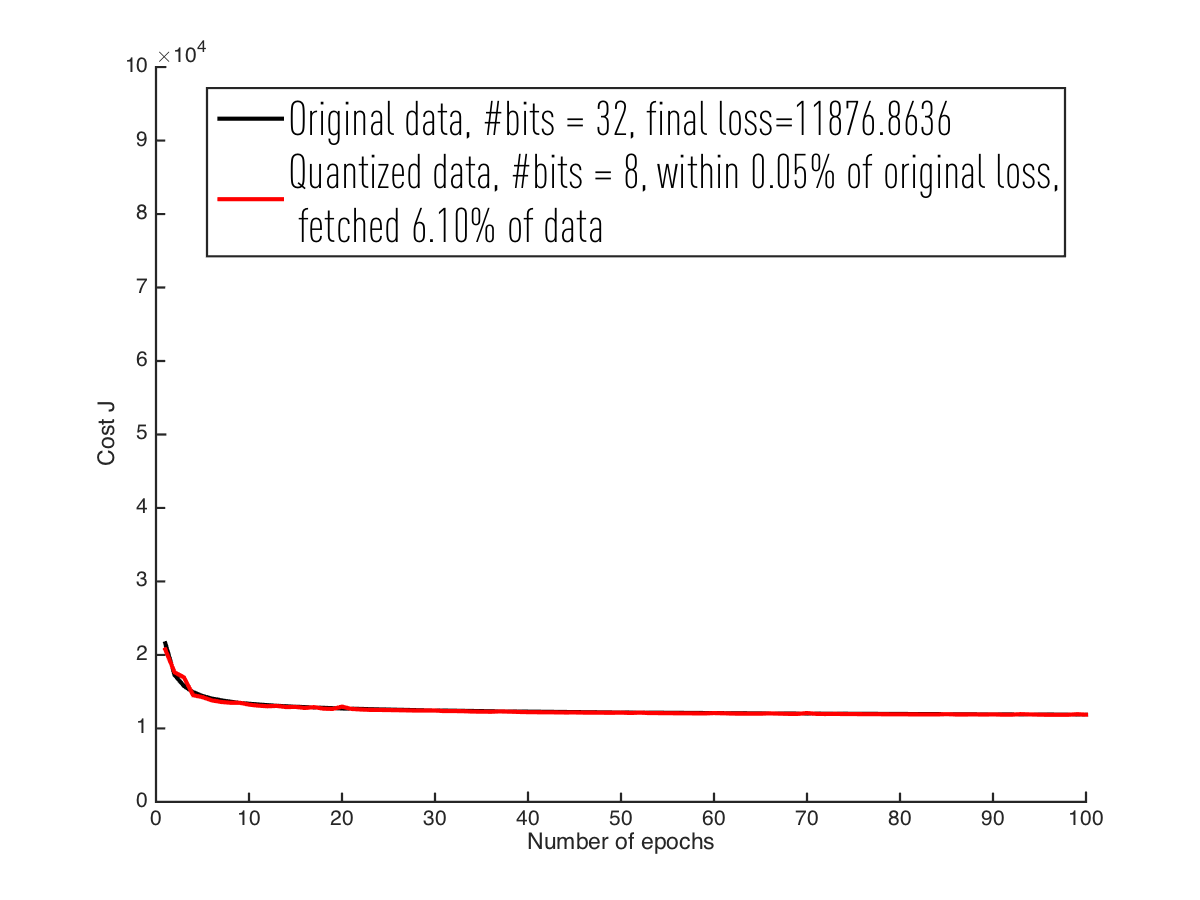
\includegraphics[width=\columnwidth]{svm/cod-rna/001}
    \caption{\texttt{cod-rna} dataset, initial stepsize = 0.01}
    \end{subfigure}
    \begin{subfigure}[b]{.3\columnwidth}
    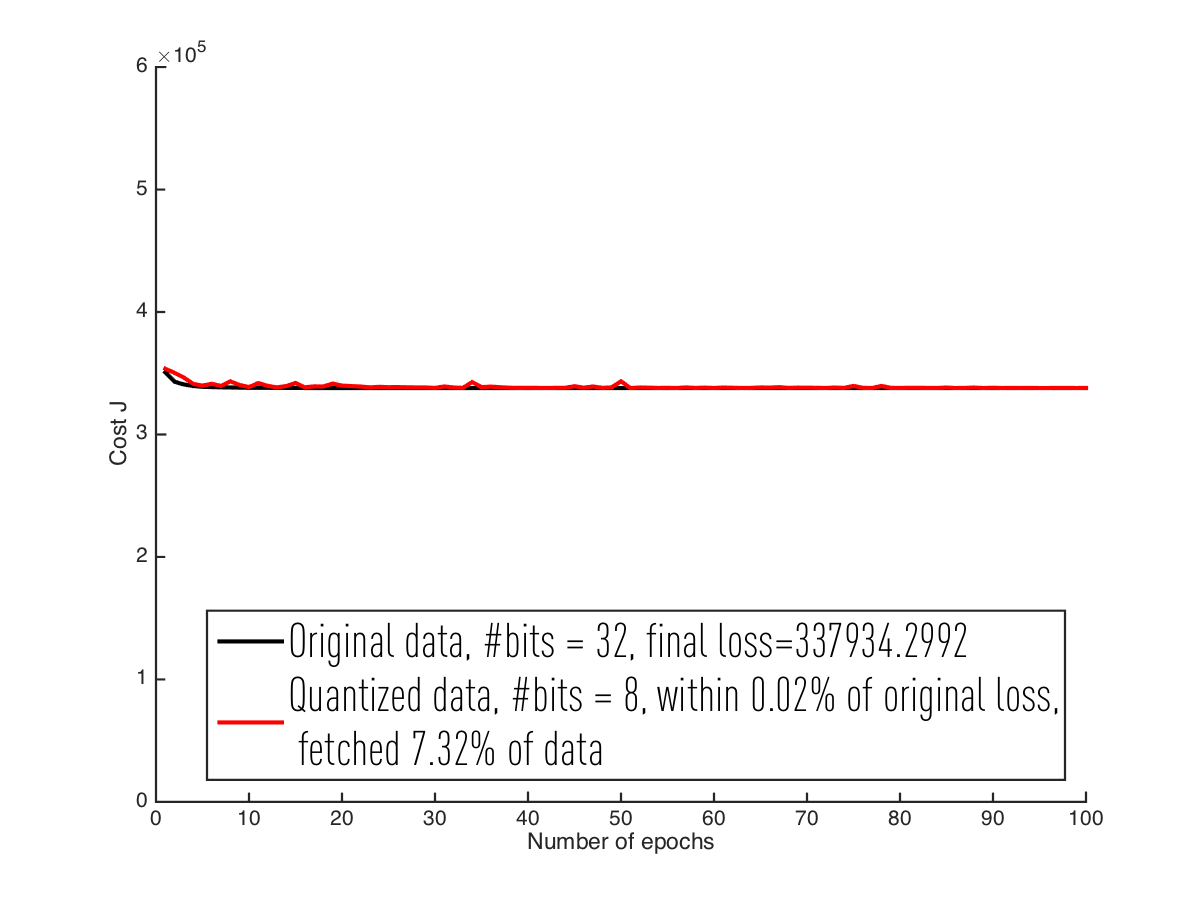
\includegraphics[width=\columnwidth]{svm/cov-type/001}
    \caption{\texttt{covtype} dataset, initial stepsize = 0.01}
    \end{subfigure}
    \begin{subfigure}[b]{.3\columnwidth}
    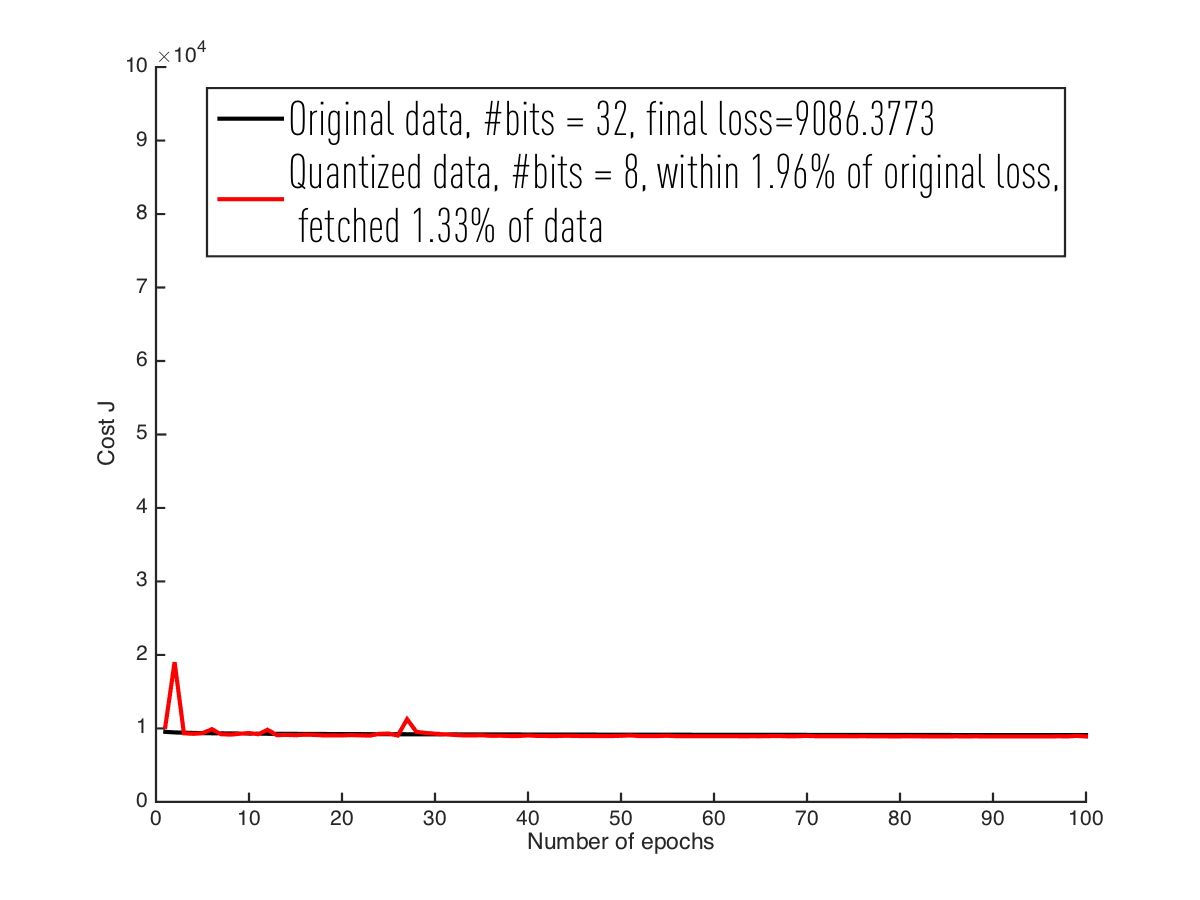
\includegraphics[width=\columnwidth]{svm/ijcnn/001}
    \caption{\texttt{ijcnn} dataset, initial stepsize = 0.01}
    \end{subfigure}
\caption{ZipML on SVM using 8-bit quantization for various datasets}
\label{fig:svm}
\end{figure}





\section{Ongoing Efforts}

%\subsection{Systems}
%
%The end-to-end low-precision representation of ZipML
%provides a range of opportunities related to system
%research. We are currently actively working
%on several system projects enabled by ZipML
%and we describe them briefly.
%
%
%\todo{Dan: How about networks? They're not really theory :) }
%
%\begin{enumerate}
%\item {\bf Hardware Primitives and Near-memory Computation.}
%ZipML's stochastic rounding scheme means that the rounding
%result for different epochs are likely to be different. In
%this scenario, an open system question is where the stochastic
%rounding procedure happens--If everytime that rounding 
%happens one need to transfer the original data from 
%memory to CPU, we do not get much benefit by using ZipML.
%Therefore, one of our ongoing projects is to design hardware primitives
%for stochastic rounding and pushes these computations
%to storage devices such as SSD and DRAM. 
%
%\item {\bf ``Machine Learning Index'' for In-Database Analytics.}
%In-Database analytics systems support training of machine
%learning models over relations (tables) stored inside 
%a relational database system (RDBMS). In RDBMS, users
%can create index such as B-Tree or hash index to speed
%up SQL queries. ZipML provides a novel way to construct
%index for ``machine learning queries'' by pre-materialize
%a set of samples and store them on disk. One of
%our ongoing projects is to understand the possibility of
%integrating this novel index into existing in-database analytics 
%systems such as Pivotal MADlib or SAP HANA PAL.
%
%\item {\bf ``Progressive Analytics''} We believe that
%ZipML provides a theoretically sound way to ``rapidly prototype''
%a machine learning model by training over low-precision
%data. One of our ongoing projects is to define and implement
%a {\em realtime}, {\em progressive}, analytics systems--Given
%10GB data, the users get a ``good enough'' model within 100ms
%to continue his follow up tasks while this model keeps
%getting refined (similar to how progressive JPEG works).
%In this way, the user does not have the feeling of waiting
%for machine learning and analytics to finish, and we believe
%this could enable a new interaction model between users and
%analytics systems.
%
%\item {\bf Edge Computing and Embedded Systems.} Many sensor
%networks in industrial environments suffer from the limitation
%of data transformation (due to power, price, and physical 
%locations). With our industrial partners, one of our
%ongoing projects is to integrate ZipML into embedded 
%systems to enable more effective data transformation 
%over sensor networks when a joint machine learning model 
%needs to be trained.
%
%\item {\bf ``Warm Storage'' Machine Learning.} Data
%involved in training a model learning model are
%often ``hot data''--they need to be put in fast storage
%such as DRAM. However, on machines whose memory bandwidth 
%is only one order
%of magnitude faster than disk bandwidth, with ZipML
%we expect to
%observe the training time to be similar no matter
%the data is on disk or in memory. We empirically validated
%this on  EC2 \texttt{c4.8xlarge} instance. This
%implies that the operating cost of machine learning
%cloud services such as Azure could be significantly
%lowered by storing more data onto cheaper/colder 
%secondary  storages without the users observe much slowdown
%or any difference in training quality. Similarly,
%users can also choose to use cheaper slower storage 
%to replace the more expensive ones. One of our
%ongoing projects is to integrate ZipML to
%machine learning cloud services and understand
%its system implications.
%
%\end{enumerate}




%\subsection{Theory}

\begin{itemize}
	\item {\bf General Loss Functions.} 
	A key question in the context of our work is whether it is possible to perform sample and model quantization 
	in the context of more complex loss functions, such as hinge loss, sigmoid, logit, or rectified linear units. 
	We speculate that this might be possible by adapting the alternating direction method of multipliers (ADMM)~\cite{ADMM}, 
	or via error correction.  
	
	\item {\bf SVM with Corrupted Labels.}  
	The discussion in Section~\ref{sec:svm} suggests the following general question: 
	Does stochastic gradient descent provide any convergence guarantees if a subset of the samples considered in an iteration (the ones with low margin) have flipped labels?
	
	\item {\bf Better Coding.}  
	We currently only employ simple coding techniques. However, it is interesting to consider whether \emph{difference coding} can be employed to code the difference between two consecutive gradients, or to reduce the bandwidth overhead of double sampling.  

\iffalse
    \item {\bf Quantized Activations and Model Compression.}  
	It is also interesting to consider whether accuracy (test loss) can be preserved when the model is quantized. 
	This question is especially important in the context of \emph{model compression}, which is an active area of research.\footnote{https://petewarden.com/2016/05/03/how-to-quantize-neural-networks-with-tensorflow/}
\fi

    \item {\bf Compression/Variance Tradeoffs.} It is not clear that the trade-offs between bit width and variance increase are tight, and we currently do not analyze the dependence on the condition number of the dataset. 
    
    \item {\bf Alternative Quantizations.} The current quantization strategy is to equally partition the interval $[0, 1]$. 
    We plan to investigate whether heterogeneous intervals can reduce variance.
    
    
    
\end{itemize}







\end{document}
